\documentclass[]{article}
\usepackage{lmodern}
\usepackage{setspace}
\setstretch{1}
\usepackage{amssymb,amsmath}
\usepackage{ifxetex,ifluatex}
\usepackage{fixltx2e} % provides \textsubscript
\ifnum 0\ifxetex 1\fi\ifluatex 1\fi=0 % if pdftex
  \usepackage[T1]{fontenc}
  \usepackage[utf8]{inputenc}
\else % if luatex or xelatex
  \ifxetex
    \usepackage{mathspec}
  \else
    \usepackage{fontspec}
  \fi
  \defaultfontfeatures{Ligatures=TeX,Scale=MatchLowercase}
\fi
% use upquote if available, for straight quotes in verbatim environments
\IfFileExists{upquote.sty}{\usepackage{upquote}}{}
% use microtype if available
\IfFileExists{microtype.sty}{%
\usepackage{microtype}
\UseMicrotypeSet[protrusion]{basicmath} % disable protrusion for tt fonts
}{}
\usepackage[margin=1in]{geometry}
\usepackage{hyperref}
\PassOptionsToPackage{usenames,dvipsnames}{color} % color is loaded by hyperref
\hypersetup{unicode=true,
            pdftitle={Component response rate variation drives stability in large complex systems},
            pdfauthor={A. Bradley Duthie},
            colorlinks=true,
            linkcolor=blue,
            citecolor=Blue,
            urlcolor=Blue,
            breaklinks=true}
\urlstyle{same}  % don't use monospace font for urls
\usepackage{color}
\usepackage{fancyvrb}
\newcommand{\VerbBar}{|}
\newcommand{\VERB}{\Verb[commandchars=\\\{\}]}
\DefineVerbatimEnvironment{Highlighting}{Verbatim}{commandchars=\\\{\}}
% Add ',fontsize=\small' for more characters per line
\usepackage{framed}
\definecolor{shadecolor}{RGB}{248,248,248}
\newenvironment{Shaded}{\begin{snugshade}}{\end{snugshade}}
\newcommand{\KeywordTok}[1]{\textcolor[rgb]{0.13,0.29,0.53}{\textbf{{#1}}}}
\newcommand{\DataTypeTok}[1]{\textcolor[rgb]{0.13,0.29,0.53}{{#1}}}
\newcommand{\DecValTok}[1]{\textcolor[rgb]{0.00,0.00,0.81}{{#1}}}
\newcommand{\BaseNTok}[1]{\textcolor[rgb]{0.00,0.00,0.81}{{#1}}}
\newcommand{\FloatTok}[1]{\textcolor[rgb]{0.00,0.00,0.81}{{#1}}}
\newcommand{\ConstantTok}[1]{\textcolor[rgb]{0.00,0.00,0.00}{{#1}}}
\newcommand{\CharTok}[1]{\textcolor[rgb]{0.31,0.60,0.02}{{#1}}}
\newcommand{\SpecialCharTok}[1]{\textcolor[rgb]{0.00,0.00,0.00}{{#1}}}
\newcommand{\StringTok}[1]{\textcolor[rgb]{0.31,0.60,0.02}{{#1}}}
\newcommand{\VerbatimStringTok}[1]{\textcolor[rgb]{0.31,0.60,0.02}{{#1}}}
\newcommand{\SpecialStringTok}[1]{\textcolor[rgb]{0.31,0.60,0.02}{{#1}}}
\newcommand{\ImportTok}[1]{{#1}}
\newcommand{\CommentTok}[1]{\textcolor[rgb]{0.56,0.35,0.01}{\textit{{#1}}}}
\newcommand{\DocumentationTok}[1]{\textcolor[rgb]{0.56,0.35,0.01}{\textbf{\textit{{#1}}}}}
\newcommand{\AnnotationTok}[1]{\textcolor[rgb]{0.56,0.35,0.01}{\textbf{\textit{{#1}}}}}
\newcommand{\CommentVarTok}[1]{\textcolor[rgb]{0.56,0.35,0.01}{\textbf{\textit{{#1}}}}}
\newcommand{\OtherTok}[1]{\textcolor[rgb]{0.56,0.35,0.01}{{#1}}}
\newcommand{\FunctionTok}[1]{\textcolor[rgb]{0.00,0.00,0.00}{{#1}}}
\newcommand{\VariableTok}[1]{\textcolor[rgb]{0.00,0.00,0.00}{{#1}}}
\newcommand{\ControlFlowTok}[1]{\textcolor[rgb]{0.13,0.29,0.53}{\textbf{{#1}}}}
\newcommand{\OperatorTok}[1]{\textcolor[rgb]{0.81,0.36,0.00}{\textbf{{#1}}}}
\newcommand{\BuiltInTok}[1]{{#1}}
\newcommand{\ExtensionTok}[1]{{#1}}
\newcommand{\PreprocessorTok}[1]{\textcolor[rgb]{0.56,0.35,0.01}{\textit{{#1}}}}
\newcommand{\AttributeTok}[1]{\textcolor[rgb]{0.77,0.63,0.00}{{#1}}}
\newcommand{\RegionMarkerTok}[1]{{#1}}
\newcommand{\InformationTok}[1]{\textcolor[rgb]{0.56,0.35,0.01}{\textbf{\textit{{#1}}}}}
\newcommand{\WarningTok}[1]{\textcolor[rgb]{0.56,0.35,0.01}{\textbf{\textit{{#1}}}}}
\newcommand{\AlertTok}[1]{\textcolor[rgb]{0.94,0.16,0.16}{{#1}}}
\newcommand{\ErrorTok}[1]{\textcolor[rgb]{0.64,0.00,0.00}{\textbf{{#1}}}}
\newcommand{\NormalTok}[1]{{#1}}
\usepackage{longtable,booktabs}
\usepackage{graphicx,grffile}
\makeatletter
\def\maxwidth{\ifdim\Gin@nat@width>\linewidth\linewidth\else\Gin@nat@width\fi}
\def\maxheight{\ifdim\Gin@nat@height>\textheight\textheight\else\Gin@nat@height\fi}
\makeatother
% Scale images if necessary, so that they will not overflow the page
% margins by default, and it is still possible to overwrite the defaults
% using explicit options in \includegraphics[width, height, ...]{}
\setkeys{Gin}{width=\maxwidth,height=\maxheight,keepaspectratio}
\IfFileExists{parskip.sty}{%
\usepackage{parskip}
}{% else
\setlength{\parindent}{0pt}
\setlength{\parskip}{6pt plus 2pt minus 1pt}
}
\setlength{\emergencystretch}{3em}  % prevent overfull lines
\providecommand{\tightlist}{%
  \setlength{\itemsep}{0pt}\setlength{\parskip}{0pt}}
\setcounter{secnumdepth}{0}
% Redefines (sub)paragraphs to behave more like sections
\ifx\paragraph\undefined\else
\let\oldparagraph\paragraph
\renewcommand{\paragraph}[1]{\oldparagraph{#1}\mbox{}}
\fi
\ifx\subparagraph\undefined\else
\let\oldsubparagraph\subparagraph
\renewcommand{\subparagraph}[1]{\oldsubparagraph{#1}\mbox{}}
\fi

%%% Use protect on footnotes to avoid problems with footnotes in titles
\let\rmarkdownfootnote\footnote%
\def\footnote{\protect\rmarkdownfootnote}

%%% Change title format to be more compact
\usepackage{titling}

% Create subtitle command for use in maketitle
\newcommand{\subtitle}[1]{
  \posttitle{
    \begin{center}\large#1\end{center}
    }
}

\setlength{\droptitle}{-2em}
  \title{Component response rate variation drives stability in large complex
systems}
  \pretitle{\vspace{\droptitle}\centering\huge}
  \posttitle{\par}
  \author{A. Bradley Duthie (
\href{mailto:alexander.duthie@stir.ac.uk}{\nolinkurl{alexander.duthie@stir.ac.uk}}
)}
  \preauthor{\centering\large\emph}
  \postauthor{\par}
  \predate{\centering\large\emph}
  \postdate{\par}
  \date{Biological and Environmental Sciences, University of Stirling, Stirling,
UK, FK9 4LA}

\usepackage{amsmath}
\usepackage{natbib}
\usepackage[utf8]{inputenc}
\bibliographystyle{amnatnat}

\begin{document}
\maketitle

\textbf{The stability of a complex system generally decreases with
increasing system size and interconnectivity, a counterintuitive result
of widespread importance across the physical, life, and social sciences.
Despite recent interest in the relationship between system properties
and stability, the effect of variation in the response rate of
individual system components remains unconsidered. Here I vary the
component response rates (\(\boldsymbol{\gamma}\)) of randomly generated
complex systems. I show that when component response rates vary, the
potential for system stability is markedly increased. Variation in
\(\boldsymbol{\gamma}\) becomes increasingly important as system size
increases, such that the largest stable complex systems would be
unstable if not for \(\boldsymbol{Var(\gamma)}\). My results reveal a
previously unconsidered driver of system stability that is likely to be
pervasive across all complex systems.}

In 1972, May\textsuperscript{\protect\hyperlink{ref-May1972}{1}} first
demonstrated that randomly assembled systems of sufficient complexity
are almost inevitably unstable given infinitesimally small
perturbations. Complexity in this case is defined by the size of the
system (i.e., the number of potentially interacting components; \(S\)),
its connectance (i.e., the probability that one component will interact
with another; \(C\)), and the variance of interaction strengths
(\(\sigma^{2}\))\textsuperscript{\protect\hyperlink{ref-Allesina2012}{2}}.
May's finding that the probability of local stability falls to near zero
given a sufficiently high threshold of \(\sigma\sqrt{SC}\) is broadly
relevant for understanding the dynamics and persistence of systems such
as
ecological\textsuperscript{\protect\hyperlink{ref-May1972}{1}--\protect\hyperlink{ref-Grilli2017}{5}},
neurological\textsuperscript{\protect\hyperlink{ref-Gray2008}{6},\protect\hyperlink{ref-Gray2009}{7}},
biochemical\textsuperscript{\protect\hyperlink{ref-Rosenfeld2009}{8},\protect\hyperlink{ref-MacArthur2010}{9}},
and
socio-economic\textsuperscript{\protect\hyperlink{ref-May2008}{10}--\protect\hyperlink{ref-Bardoscia2017}{13}}
networks. As such, identifying general principles that drive stability
in complex systems is of wide-ranging importance.

Randomly assembled complex systems can be represented as large square
matrices (\(\mathbf{M}\)) with \(S\) components (e.g., networks of
species\textsuperscript{\protect\hyperlink{ref-Allesina2012}{2}} or
banks\textsuperscript{\protect\hyperlink{ref-Haldane2011}{11}}). One
element of such a matrix, \(M_{ij}\), defines how component \(j\)
affects component \(i\) in the system at a point of
equilibrium\textsuperscript{\protect\hyperlink{ref-Allesina2012}{2}}.
Off-diagonal elements (\(i \neq j\)) therefore define interactions
between components, while diagonal elements (\(i = j\)) define component
self-regulation (e.g., carrying capacity in ecological communities).
Traditionally, off-diagonal elements are assigned non-zero values with a
probability \(C\), which are sampled from a distribution with variance
\(\sigma^{2}\); diagonal elements are set to
-1\textsuperscript{\protect\hyperlink{ref-May1972}{1},\protect\hyperlink{ref-Allesina2012}{2},\protect\hyperlink{ref-Allesina2015}{4}}.
Local system stability is assessed using eigenanalysis, with the system
being stable if the real parts of all eigenvalues (\(\lambda\)) of
\(\mathbf{M}\) are negative
(\(\max\left(\Re(\lambda)\right) < 0\))\textsuperscript{\protect\hyperlink{ref-May1972}{1},\protect\hyperlink{ref-Allesina2012}{2}}.
In a large system (high \(S\)), eigenvalues are distributed
uniformly\textsuperscript{\protect\hyperlink{ref-Tao2010}{14}} within a
circle centred at \(\Re = -1\) (the mean value of diagonal elements) and
\(\Im = 0\), with a radius of
\(\sigma\sqrt{SC}\)\textsuperscript{\protect\hyperlink{ref-May1972}{1},\protect\hyperlink{ref-Allesina2012}{2},\protect\hyperlink{ref-Allesina2015}{4}}
(Figs 1a and 2a). Local stability of randomly assembled systems
therefore becomes increasingly unlikely as \(S\), \(C\), and
\(\sigma^{2}\) increase.

May's\textsuperscript{\protect\hyperlink{ref-May1972}{1},\protect\hyperlink{ref-Allesina2012}{2}}
stability criterion \(\sigma\sqrt{SC} < 1\) assumes that individual
components respond to perturbations of the system at the same rate
(\(\gamma\)), but this is highly unlikely in any complex system. In
ecological communities, for example, the rate at which population
density changes following perturbation will depend on the generation
time of organisms, which might vary by orders of magnitude among
species. Species with short generation times will respond quickly (high
\(\gamma\)) to perturbations relative to species with long generation
times (low \(\gamma\)). Similarly, the speed at which individual banks
respond to perturbations in financial networks, or individuals or
institutions respond to perturbations in complex social networks, is
likely to vary. The effect of such variance on stability has not been
investigated in complex systems theory. Intuitively, variation in
\(\gamma\) might be expected to decrease system stability by introducing
a new source of variation into the system and thereby increasing
\(\sigma\). Here I show why, despite higher \(\sigma\), complex systems
in which \(\gamma\) varies are actually more likely to be stable,
especially when \(S\) is high.

\subsection{Results}\label{results}

\textbf{Component response rates of random complex systems}. Rows in
\(\mathbf{M}\) define how a given component \(i\) is affected by other
components of the system, meaning that the rate of component response
time can be modelled by multiplying all row elements by a real scalar
value
\(\gamma_{i}\)\textsuperscript{\protect\hyperlink{ref-Patel2018}{15}}.
The distribution of \(\gamma\) over \(S\) components thereby models the
distribution of component response rates. An instructive example
compares one \(\mathbf{M}\) where \(\gamma_{i} = 1\) for all \(i\) in
\(S\) to the same \(\mathbf{M}\) when half of \(\gamma_{i} = 1.95\) and
half of \(\gamma_{i} = 0.05\). This models one system in which
\(\gamma\) is invariant and one in which \(\gamma\) varies, but systems
are otherwise identical (note \(E[\gamma_{i}] = 1\) in both cases). I
assume \(S = 200\), \(C = 0.05\), and \(\sigma = 0.4\); diagonal
elements are set to \(-1\) and non-zero off-diagonal elements are drawn
randomly from \(\mathcal{N}(0, \sigma^{2})\). Rows are then multiplied
by \(\gamma_{i}\) to generate \(\mathbf{M}\). When \(\gamma_{i} = 1\),
eigenvalues of \(\mathbf{M}\) are distributed uniformly within a circle
centred at (\(-1, 0\)) with a radius of 1.265 (Fig. 1a). Hence, the real
components of eigenvalues are highly unlikely to all be negative when
all \(\gamma_{i} = 1\). But when \(\gamma_{i}\) values are separated
into two groups, eigenvalues are no longer uniformly distributed (Fig.
1b). Instead, two distinct clusters of eigenvalues appear (red circles
in Fig. 1b), one centred at (\(-1.95, 0\)) and the other centred at
(\(-0.05, 0\)). The former has a large radius, but the real components
have shifted to the left (in comparison to when \(\gamma = 1\)), while
the latter cluster has a smaller radius, but real components have
shifted to the right; all \(\Re({\lambda}) < 0\). Overall, for 1 million
randomly assembled \(\mathbf{M}\), this division between slow and fast
component response rates results in more stable systems: 1 stable given
\(\gamma = 1\) versus 32 stable given \(\gamma = \{1.95, 0.5\}\).

Higher stability in systems with variation in \(\gamma\) can be observed
by sampling \(\gamma_{i}\) values from various distributions. I focus on
a uniform distribution where \(\gamma \sim \mathcal{U}(0, 2)\) (see
Supplementary Information for other distributions, which give similar
results). As with the case of \(\gamma = \{1.95, 0.5\}\) (Fig. 1b),
\(E[\gamma] = 1\) when \(\gamma \sim \mathcal{U}(0, 2)\), allowing
comparison of \(\mathbf{M}\) before and after the addition of variation
in component response rate. Figure 2 shows a comparison of eigenvalue
distributions given \(S = 1000\), \(C = 0.05\), and \(\sigma = 0.4\). As
expected\textsuperscript{\protect\hyperlink{ref-Tao2010}{14}}, when
\(\gamma = 1\), eigenvalues are distributed uniformly in a circle
centred at (\(-1, 0\)) with a radius of \(\sigma\sqrt{SC} =\) 2.828.
Uniform variation in \(\gamma\) leads to a non-uniform distribution of
eigenvalues\textsuperscript{\protect\hyperlink{ref-Ahmadian2015}{16}--\protect\hyperlink{ref-Stone2017}{18}},
some of which are clustered locally near the centre of the distribution,
but others of which are spread outside the former radius of 2.828 (Fig
2b). The clustering and spreading of eigenvalues introduced by
\(Var(\gamma)\) can destabilise previously stable systems or stabilise
systems that are otherwise unstable. But where systems are otherwise too
complex to be stable given \(\gamma = 1\), the effect of \(Var(\gamma)\)
can often lead to stability above
May's\textsuperscript{\protect\hyperlink{ref-May1972}{1},\protect\hyperlink{ref-Allesina2012}{2}}
threshold \(\sigma\sqrt{SC} < 1\).

\textbf{Simulation of random \(\mathbf{M}\) across \(\mathbf{S}\)}. To
investigate the effect of \(Var(\gamma)\) on system stability, I
simulated random \(\mathbf{M}\) matrices at \(\sigma = 0.4\) and
\(C = 1\) across \(S = \{2, 3, ..., 49, 50\}\). One million
\(\mathbf{M}\) were simulated for each \(S\), and the stability of
\(\mathbf{M}\) was assessed given \(\gamma = 1\) versus
\(\gamma \sim \mathcal{U}(0, 2)\). For all \(S > 10\), I found that the
number of stable random systems was higher given \(Var(\gamma)\) than
when \(\gamma = 1\) (Fig. 3; see Supplementary Information for full
table of results), and that the difference between the probabilities of
observing a stable system increased with an increase in \(S\); i.e., the
potential for \(Var(\gamma)\) to drive stability increased with system
complexity. For the highest values of \(S\), nearly all systems that
were stable given \(Var(\gamma)\) would not have been stable given
\(\gamma = 1\).

\textbf{Targeted manipulation of \(\mathbf{\gamma}\)}. To further
investigate the potential of \(Var(\gamma)\) to be stabilising, I used a
genetic algorithm. Genetic algorithms are heuristic tools that mimic
evolution by natural selection, and are useful when the space of
potential solutions (in this case, possible combinations of \(\gamma\)
values leading to stability in a large complex system) is too large to
search
exhaustively\textsuperscript{\protect\hyperlink{ref-Hamblin2013}{19}}.
Generations of selection on \(\gamma\) value combinations to minimise
\(\max\left(\Re(\lambda)\right)\) demonstrated the potential for
\(Var(\gamma)\) to increase system stability. Across
\(S = \{2, 3, ..., 39, 40\}\), sets of \(\gamma\) values were found that
resulted in stable systems with probabilities that were up to four
orders of magnitude higher than when \(\gamma = 1\) (Fig. 4), meaning
that stability could often be achieved by manipulating \(S\) \(\gamma\)
values rather than \(S \times S\) \(\mathbf{M}\) elements.

\textbf{System feasibility given \(\mathbf{Var(\gamma)}\)} For complex
systems in which individual system components represent the density of
some tangible quantity, it is relevant to consider the feasibility of
the system. Feasibilility assumes that the system is stable and values
of all components are positive at
equilibrium\textsuperscript{\protect\hyperlink{ref-Grilli2017}{5},\protect\hyperlink{ref-Dougoud2018}{20},\protect\hyperlink{ref-Song2018}{21}}.
This is of particular interest for ecological communities because
population density cannot take negative values, meaning that ecological
systems need to be feasible for stability to be biologically
realistic\textsuperscript{\protect\hyperlink{ref-Dougoud2018}{20}}.
While my results are intended to be general to all complex systems, and
not restricted to species networks, I have also performed a feasibility
analysis on all matrices \(\mathbf{M}\) tested for stability, and
additionally for specific types of ecological
communities\textsuperscript{\protect\hyperlink{ref-Allesina2012}{2}}
(e.g., competitive, mutualist, predator-prey; see Supplementary
Information). Feasibility was unaffected by \(Var(\gamma)\), meaning
that for pure interacting species networks, variation in component
response rate (i.e., species generation time) does not affect stability
at biologically realistic species densities.

\begin{center}\rule{0.5\linewidth}{\linethickness}\end{center}

\textbf{Figure 1: Example distribution of eigenvalues before (a) and
after (b) separating a randomly generated complex system into fast
(\(\boldsymbol{\gamma} = 1.95\)) and slow
(\(\boldsymbol{\gamma} = 0.05\)) component response rates.} Each panel
shows the same system where \(S = 200\), \(C = 0.05\), and
\(\sigma = 0.4\), and in each case \(E[\gamma] = 1\) (i.e., only the
distribution of \(\gamma\) differs between panels). \textbf{a.}
Eigenvalues plotted when all \(\gamma = 1\); distributions of points are
uniformly distributed within the blue circle with a radius of
\(\sigma\sqrt{SC} =\) 1.238 centred at -1 on the real axis. \textbf{b.}
Eigenvalues plotted when half \(\gamma = 1.95\) and half
\(\gamma = 0.05\); distributions of points can be partitioned into one
large circle centred at \(\gamma = -1.95\) and one small circle centred
at \(\gamma = -0.05\). In a, the maximum real eigenvalue
\(\max\left(\Re(\lambda)\right) =\) 0.2344871, while in b
\(\max\left(\Re(\lambda)\right) =\) -0.0002273135, meaning that the
complex system in b but not a is stable because in b
\(\max\left(\Re(\lambda)\right) < 0\). In 1 million randomly generated
complex systems under the same parameter values, 1 was stable when
\(\gamma = 1\) while 32 were stable when \(\gamma = \{1.95, 0.05\}\).
Overall, complex systems that are separated into fast versus slow
components tend to be more stable than otherwise identical systems with
identical component response rates.

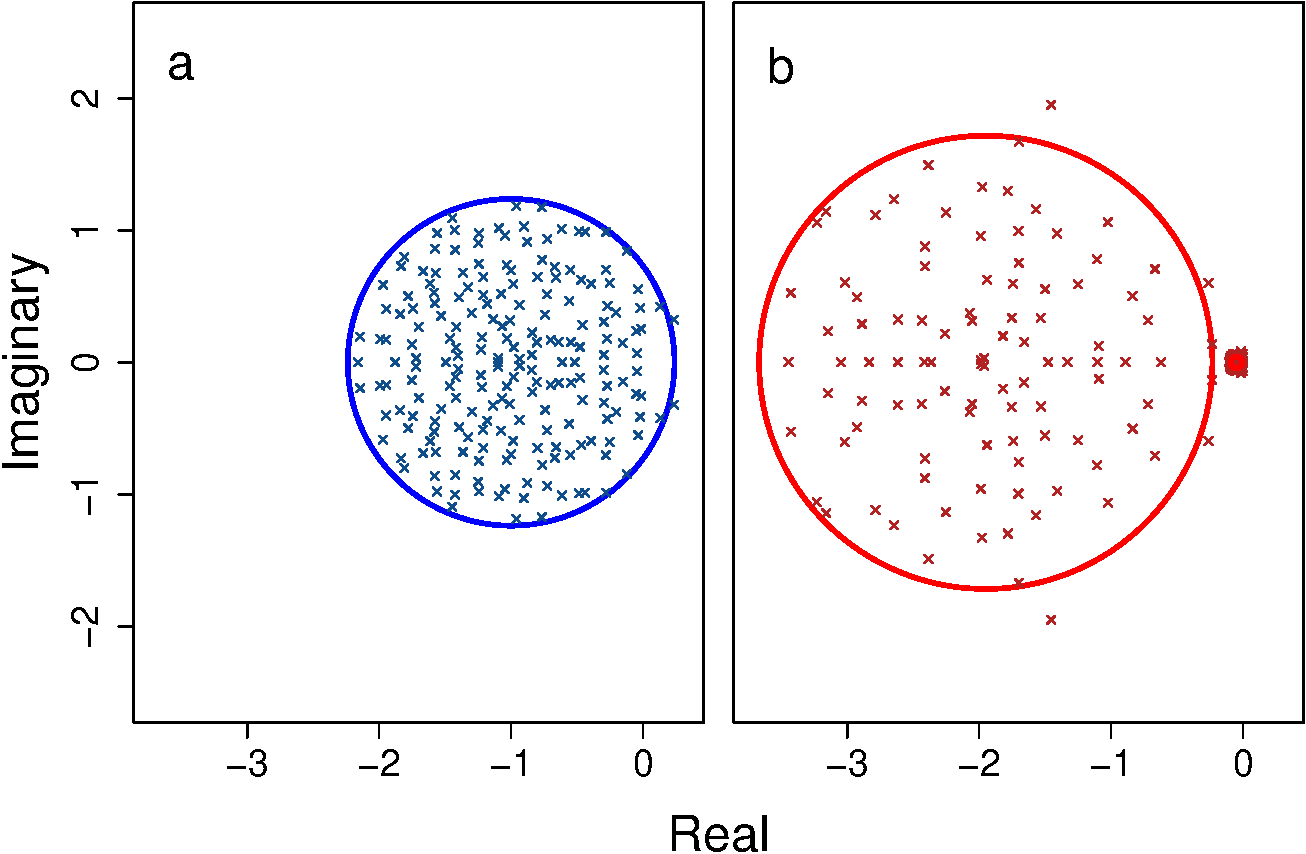
\includegraphics{unnamed-chunk-10-1.pdf}

\begin{center}\rule{0.5\linewidth}{\linethickness}\end{center}

\subsection{Discussion}\label{discussion}

Here I have shown that the stability of large systems might often be
contigent upon variation in the response rates of their individual
components, meaning that factors such as rate of trait evolution (in
biological networks), transaction speed (in economic networks), or
communication speed (in social networks) need to be considered when
investigating the stability of complex systems. Variation in component
response rate becomes more likely to be critical for stability as system
size increases, and can ultimately increase the overall probability that
system stability is observed above that predicted by
May's\textsuperscript{\protect\hyperlink{ref-May1972}{1}} classically
derived \(\sigma \sqrt{SC}\) criterion. The logic outlined here is
general, and potentially applies to any complex system in which
individual system components can vary in their reaction rates to system
perturbation.

\begin{center}\rule{0.5\linewidth}{\linethickness}\end{center}

\textbf{Figure 2: Distributions of eigenvalues before (a) and after (b)
introducing variation in component response rate
(\(\boldsymbol{\gamma}\)) in complex systems.} Each panel show the same
system where \(S = 1000\), \(C = 0.05\), and \(\sigma = 0.4\).
\textbf{a.} Eigenvalues plotted in the absence of \(Var(\gamma)\) where
\(E[\gamma] = 1\), versus \textbf{b.} eigenvalues plotted given
\(\gamma \sim \mathcal{U}(0, 2)\), which increases the variance of
interaction strengths (\(\sigma^{2}\)) but also creates a cluster of
eigenvalues toward the distribution's centre (-1, 0). Blue elipses in
both panels show the circle centred on the distribution in panel a.
Proportions of \(\Re(\lambda) < 0\) are 0.719 and 0.735 for a and b,
respectively.

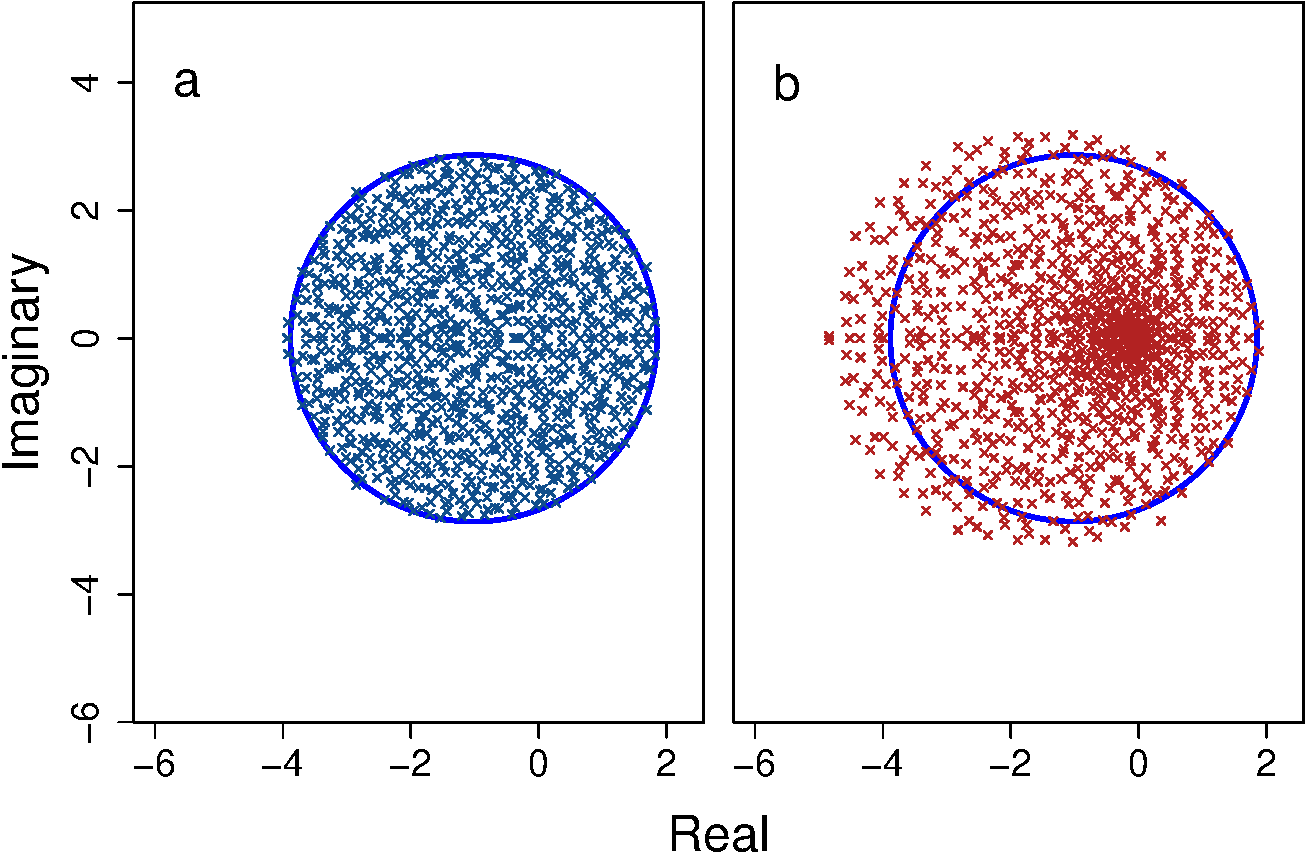
\includegraphics{unnamed-chunk-13-1.pdf}

\begin{center}\rule{0.5\linewidth}{\linethickness}\end{center}

It is important to emphasise that variation in component response rate
is not stabilising per se; that is, adding variation in component
response rate to a particular system does not necessarily increase the
probability that the system will be stable. Rather, systems that are
observed to be stable are more likely to have varying component response
rates, and for this variation to be critical to their stability (Fig.
3). This is caused by the shift to a non-uniform distribution of
eigenvalues that occurs by introducing \(Var(\gamma)\) (Fig. 1b, 2b),
which can sometimes cause all of the real components of the eigenvalues
of the community matrix \(\mathbf{M}\) to become negative, but might
also increase the real components of eigenvalues. The mathematics
underlying this shift in eigenvalue distribution has been
investigated\textsuperscript{\protect\hyperlink{ref-Ahmadian2015}{16}}
and recently applied to questions concerning species density and
feasibility\textsuperscript{\protect\hyperlink{ref-Gibbs2017}{17},\protect\hyperlink{ref-Stone2017}{18}},
but has not been interpreted as rates of response of individual system
components to perturbation.

The potential importance of component response rate variation was most
evident from the results of simulations in which the genetic algorithm
was used in attempt to maximise the probability of system stability. The
probability that some combination of component response rates could be
found to stabilise the system was shown to be up to four orders of
magnitude higher than the background probabilities of stability in the
absence of any component response rate variation. Instead of
manipulating the \(S \times S\) interactions between system components,
it might therefore be possible to manipulate only the \(S\) response
rates of individual system components to achieve stability. Hence,
managing the response rates of system components in a targeted way could
potentially facilitate the stabilisation of complex systems through a
reduction in dimensionality.

\begin{center}\rule{0.5\linewidth}{\linethickness}\end{center}

\textbf{Figure 3: Stability of large complex systems with and without
variation in component response rate (\(\boldsymbol{\gamma}\)).} The
\(\ln\) number of systems that are stable across different system sizes
(\(S\), max \(S=50\)) given \(C = 1\), and the proportion of systems in
which variation in \(\gamma\) is critical for system stability. For each
\(S\), 1 million complex systems are randomly generated. Stability of
each complex system is tested given variation in \(\gamma\) by randomly
sampling \(\gamma \sim \mathcal{U}(0, 2)\). Stability given
\(Var(\gamma)\) is then compared to stability in an otherwise identical
system in which \(\gamma = E[\mathcal{U}(0, 2)]\) for all components.
Blue and red bars show the number of stable systems in the absence and
presence of \(Var(\gamma)\), respectively. The black line shows the
proportion of systems that are stable when \(Var(\gamma) > 0\), but
would be unstable if \(Var(\gamma) = 0\).

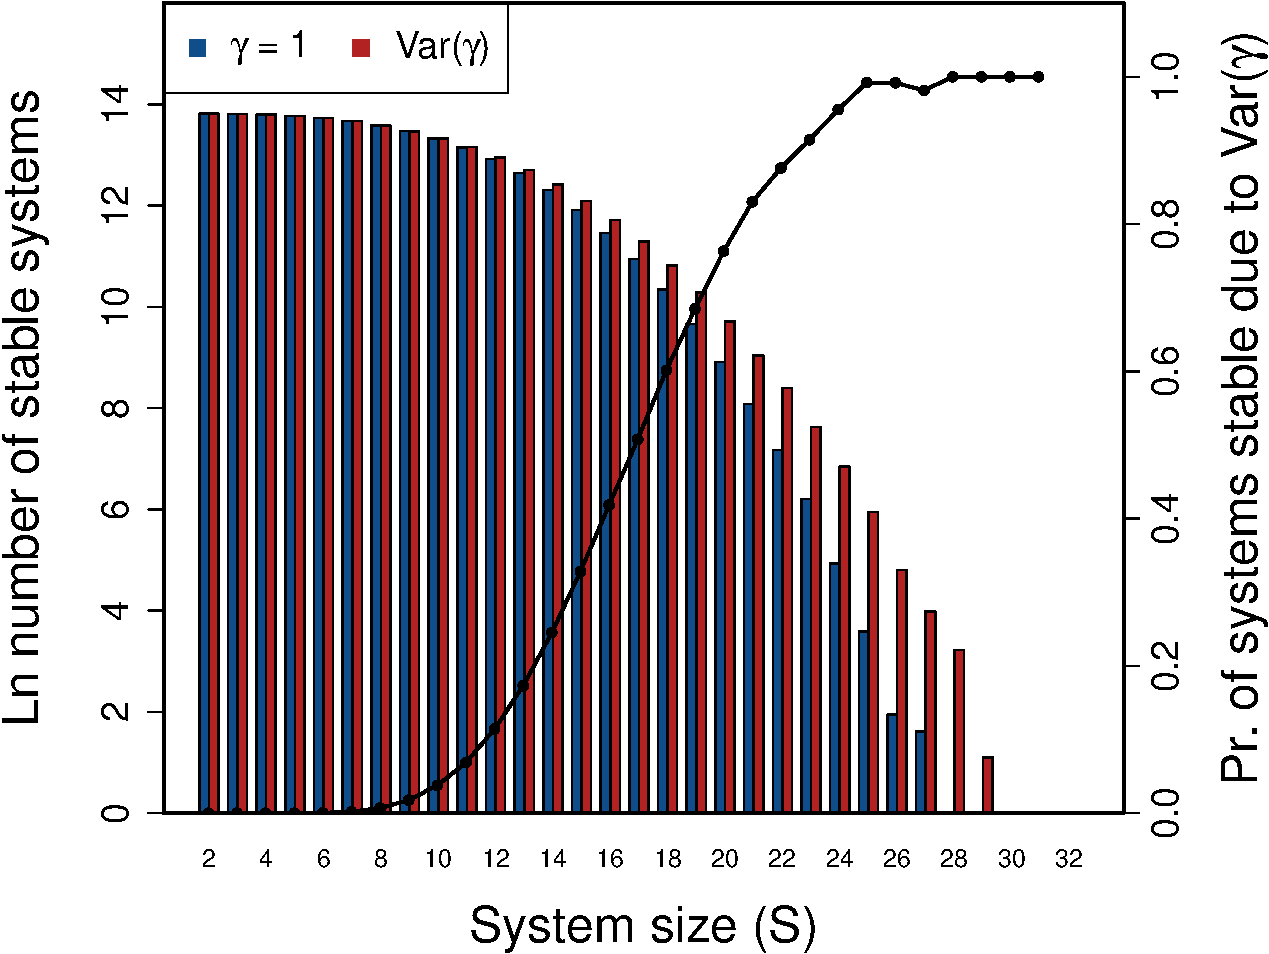
\includegraphics{unnamed-chunk-15-1.pdf}

\begin{center}\rule{0.5\linewidth}{\linethickness}\end{center}

Interestingly, while complex systems were more likely to be stable given
variation in component response rate, they were not more likely to be
feasible, meaning that stability was not increased when component values
were also restricted to being positive at equilibrium. Feasibility is
important to consider, particularly for the study of ecological networks
of
species\textsuperscript{\protect\hyperlink{ref-Grilli2017}{5},\protect\hyperlink{ref-Stone2017}{18},\protect\hyperlink{ref-Dougoud2018}{20}}
because population densities cannot realistically be negative. My
results therefore suggest that variation in the rate of population
responses to perturbation (e.g., due to differences in generation time
among species) is unlikely to be critical to the stability of purely
multi-species interaction networks (see also Supplementary Information).
Nevertheless, ecological interactions do not exist in isolation in
empirical
systems\textsuperscript{\protect\hyperlink{ref-Patel2018}{15}}, but
instead interact with evolutionary, abiotic, or social-economic systems.
The relevance of component response rate for complex system stability
should therefore not be ignored in the broader context of ecological
communities.

\begin{center}\rule{0.5\linewidth}{\linethickness}\end{center}

\textbf{Figure 4: Stability of large complex systems given
\(\boldsymbol{\gamma = 1}\) versus targeted
\(\boldsymbol{Var(\gamma)}\).} The \(\ln\) number of systems that are
stable across different system sizes (\(S\), max \(S=40\)) for
\(C = 1\), and the proportion of systems wherein a targeted search of
\(\gamma\) values successfully resulted in system stability. For each
\(S\), 100000 complex systems are randomly generated. Stability of each
complex system is tested given variation in \(\gamma\) using a genetic
algorithm to maximise the effect of \(\gamma\) values on increasing
stability, as compared to stability in an otherwise identical system in
which \(\gamma\) is the same for all components. Blue bars show the
number of stable systems in the absence of component response rate
variation, while red bars show the number of stable systems that can be
generated if component response rate is varied to maximise system
stability. The black line shows the proportion of systems that are
stable when component response rate is targeted to increase stability,
but would not be stable if \(Var(\gamma) = 0\).

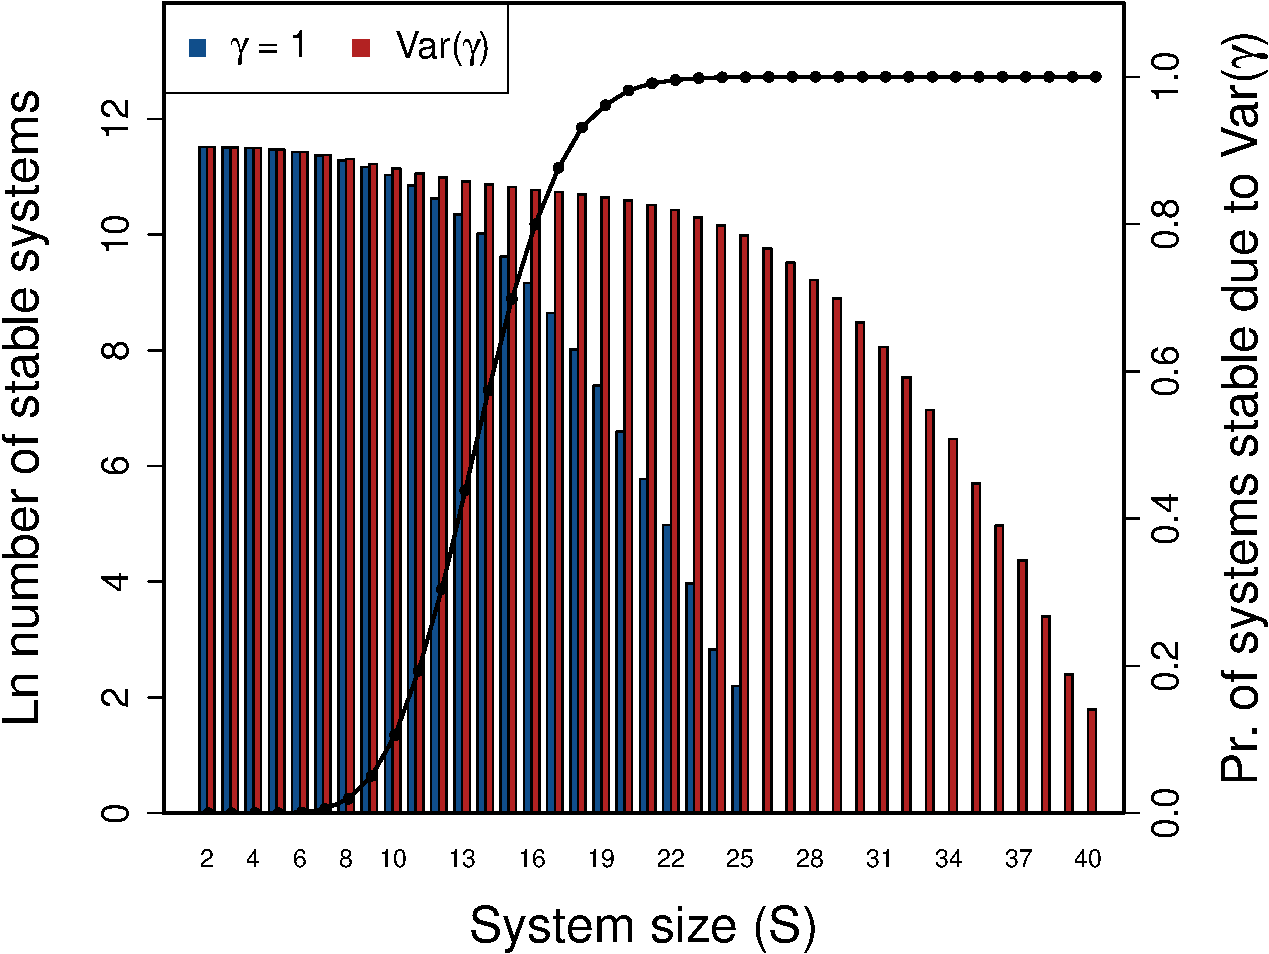
\includegraphics{unnamed-chunk-16-1.pdf}

\begin{center}\rule{0.5\linewidth}{\linethickness}\end{center}

My results show that complex systems are more likely to be stable when
the response rates of system components vary. These results are broadly
applicable to understanding stability of complex networks in the
physical, life, and social sciences.

\subsection{Methods}\label{methods}

\textbf{Component response rate variation (\(\mathbf{\gamma}\))}. In a
synthesis of eco-evolutionary feedbacks on community stability, Patel et
al. model a system that includes a vector of potentially changing
species densities (\(\mathbf{N}\)) and a vector of potentially evolving
traits
(\(\mathbf{x}\))\textsuperscript{\protect\hyperlink{ref-Patel2018}{15}}.
For any species \(i\) or trait \(j\), change in species density
(\(N_{i}\)) or trait value (\(x_{j}\)) with time (\(t\)) is a function
of the vectors \(\mathbf{N}\) and \(\mathbf{x}\),

\[\frac{dN_{i}}{dt} = N_{i}f_{i}(\mathbf{N}, \mathbf{x}),\]

\[\frac{dx_{j}}{dt} = \epsilon g_{j}(\mathbf{N}, \mathbf{x}).\]

In the above, \(f_{i}\) and \(g_{j}\) are functions that define the
effects of all species densities and trait values on the density of a
species \(i\) and the value of trait \(j\), respectively. Patel et al.
were interested in stability when the evolution of traits was relatively
slow or fast in comparison with the change in species
densities\textsuperscript{\protect\hyperlink{ref-Patel2018}{15}}, and
this is modulated in the above by the scalar \(\epsilon\). The value of
\(\epsilon\) thereby determines the timescale separation between ecology
and evolution, with high \(\epsilon\) modelling relatively fast
evolution and low \(\epsilon\) modelling relative slow
evolution\textsuperscript{\protect\hyperlink{ref-Patel2018}{15}}.

I use the same principle that Patel et al. use to modulate the relative
rate of evolution to modulate rates of component responses for \(S\)
components. Following
May\textsuperscript{\protect\hyperlink{ref-May1972}{1},\protect\hyperlink{ref-May1973}{22}},
the value of a component \(i\) at time \(t\) (\(v_{i}(t)\)) is affected
by the value of \(j\) (\(v_{j}(t)\)) and \(j\)'s marginal effect on
\(i\) (\(a_{ij}\)), and by \(i\)'s response rate (\(\gamma_{i}\)),

\[\frac{dv_{i}(t)}{dt} = \gamma_{i} \sum_{j=1}^{S}a_{ij}v_{j}(t).\]

In matrix notation\textsuperscript{\protect\hyperlink{ref-May1973}{22}},

\[\frac{d\mathbf{v}(t)}{dt} = \mathbf{\gamma} \mathbf{A}\mathbf{v}(t).\]

In the above, \(\mathbf{\gamma}\) is a diagonal matrix in which elements
correspond to individual component response rates. Therefore,
\(\mathbf{M} =\mathbf{\gamma} \mathbf{A}\) modulates the values of
components and can be analysed using the techniques of
May\textsuperscript{\protect\hyperlink{ref-May1972}{1},\protect\hyperlink{ref-Ahmadian2015}{16},\protect\hyperlink{ref-May1973}{22}}.

\textbf{Genetic algorithm}. Ideally, to investigate the potential of
\(Var(\gamma)\) for increasing the proportion of stable complex systems,
the search space of all possible \(\gamma\) vectors would be evaluated
for each unique \(\mathbf{M = \gamma A}\). This is technically
impossible because \(\gamma_{i}\) can take any real value between 0-2,
but even rounding \(\gamma_{i}\) to reasonable values would result in a
search space too large to practically explore. Under these conditions,
genetic algorithms are highly useful tools for finding practical
solutions by mimicking the process of biological
evolution\textsuperscript{\protect\hyperlink{ref-Hamblin2013}{19}}. In
this case, the practical solution is finding vectors of
\(\mathbf{\gamma}\) that decrease the most positive real eigenvalue of
\(\mathbf{M}\). The genetic algorithm used achieves this by initialising
a large population of 1000 different potential \(\mathbf{\gamma}\)
vectors and allowing this population to evolve through a process of
mutation, crossover (swaping \(\gamma_{i}\) values between vectors),
selection, and reproduction until either a \(\mathbf{\gamma}\) vector is
found where all \(\Re(\lambda) < 0\) or some ``giving up'' critiera is
met.

For each \(S = \{2, 3, ..., 39, 40\}\), the genetic algorithm was run
for 100000 random \(\mathbf{M}\) (\(\sigma = 0.4\), \(C = 1\)), where
\(\mathbf{M = \gamma A}\). The genetic algorithm was initialised with a
population of 1000 different \(\mathbf{\gamma}\) vectors with elements
sampled i.i.d from \(\gamma_{i} \sim \mathcal{U}(0, 2)\). Eigenanalysis
was performed on the \(\mathbf{M}\) resulting from each
\(\mathbf{\gamma}\) vector, and the 20 \(\mathbf{\gamma}\) vectors
resulting in \(\mathbf{M}\) with the lowest
\(\max\left(\Re(\lambda)\right)\) each produced 50 clonal offspring with
subsequent random mutation and crossover between the resulting new
generation of 1000 \(\mathbf{\gamma}\) vectors. Mutation of each
\(\gamma_{i}\) in a \(\mathbf{\gamma}\) vector occurred with a
probability of 0.2, resulting in a mutation effect of size
\(\mathcal{N}(0, 0.02)\) being added to generate the newly mutated
\(\gamma_{i}\) (any \(\gamma_{i}\) values that mutated below zero were
multiplied by \(-1\), and any values that mutated above 2 were set to
2). Crossover occurred between two sets of 100 \(\mathbf{\gamma}\)
vectors paired in each generation; vectors were randomly sampled with
replacement among but not within sets. Vector pairs selected for
crossover swapped all elements between and including two \(\gamma_{i}\)
randomly selected with replacement (this allowed for reversal of vector
element positions during crossover; e.g.,
\(\{\gamma_{4}, \gamma_{5}, \gamma_{6}, \gamma_{7}\} \to \{\gamma_{7}, \gamma_{6}, \gamma_{5}, \gamma_{4}\}\)
). The genetic algorithm terminated if a stable \(\mathbf{M}\) was
found, 20 generations occurred, or if the mean \(\mathbf{\gamma}\)
fitness increase between generations was less than 0.01 (where fitness
was defined as \(W_{\gamma} = -\max\left(\Re(\lambda)\right)\) for
\(\mathbf{M}\)).

\textbf{System feasibility}. Dougoud et
al.\textsuperscript{\protect\hyperlink{ref-Dougoud2018}{20}} define the
following feasibility criteria for ecological systems characterised by
\(S\) interacting species with varying densities in a classical
Lotka-Volterra model,

\[\mathbf{x^{*}} = -\left(\theta \mathbf{I} + (CS)^{-\delta}\mathbf{J} \right)^{-1}\mathbf{r}.\]

In the above, \(\mathbf{x^{*}}\) is the vector of species densities at
equilibrium. Feasibility is satisfied if all elements in
\(\mathbf{x^{*}}\) are positive. The matrix \(\mathbf{I}\) is the
identity matrix, and the value \(\theta\) is the strength of
intraspecific competition (diagonal elements). Diagonal values are set
to \(-1\), so \(\theta = -1\). The variable \(\delta\) is a
normalisation parameter that modulates the strength of interactions
(\(\sigma\)) for \(\mathbf{J}\). Implicitly, here \(\delta = 0\)
underlying strong interactions. Hence, \((CS)^{-\delta} = 1\), so in the
above, a diagonal matrix of -1s (\(\theta \mathbf{I}\)) is added to
\(\mathbf{J}\), which has a diagonal of all zeros and an off-diagonal
affecting species interactions (i.e., the expression \((CS)^{-\delta}\)
relates to May's\textsuperscript{\protect\hyperlink{ref-May1972}{1}}
stability
criterion\textsuperscript{\protect\hyperlink{ref-Dougoud2018}{20}} by
\(\frac{\sigma}{(CS)^{-\delta}}\sqrt{SC} < 1\), and hence for my
purposes \((CS)^{-\delta} = 1\)). Given
\(\mathbf{A} = \theta\mathbf{I + J}\), the above criteria is therefore
reduced to the below,

\[\mathbf{x^{*} = -A^{-1}r}.\]

To check the feasibility criteria for \(\mathbf{M = \gamma A}\), I
therefore evaluated \(\mathbf{-M^{-1}r}\) (\(\mathbf{r}\) elements were
sampled i.i.d. from \(r_{i} \sim \mathcal{N}(0, 0.4^{2})\)). Feasibility
is satisfied if all of the elements of the resulting vector are
positive.

\textbf{Acknowledgements:} I am supported by a Leverhulme Trust Early
Career Fellowship (ECF-2016-376). Conversations with L. Bussière and N.
Bunnefeld, and comments from J. J. Cusack and I. L. Jones, improved the
quality of this work.

\textbf{Supplementary Information:} Full tables of stability results for
simulations across different system size (\(S\)) values, ecological
community types, connectance (\(C\)) values, interaction strengths
(\(\sigma\)), and \(\gamma\) distributions are provided as supplementary
material. An additional table also shows results for how feasibility
changes across \(S\). All code and simulation outputs are publicly
available as part of the RandomMatrixStability package on GitHub
(\url{https://github.com/bradduthie/RandomMatrixStability}).

\textbf{References}

\hypertarget{refs}{}
\hypertarget{ref-May1972}{}
1. May, R. M. Will a large complex system be stable? \emph{Nature}
\textbf{238,} 413--414 (1972).

\hypertarget{ref-Allesina2012}{}
2. Allesina, S. \& Tang, S. Stability criteria for complex ecosystems.
\emph{Nature} \textbf{483,} 205--208 (2012).

\hypertarget{ref-Mougi2012}{}
3. Mougi, A. \& Kondoh, M. Diversity of interaction types and ecological
community stability. \emph{Science} \textbf{337,} 349--351 (2012).

\hypertarget{ref-Allesina2015}{}
4. Allesina, S. \emph{et al.} Predicting the stability of large
structured food webs. \emph{Nature Communications} \textbf{6,} 7842
(2015).

\hypertarget{ref-Grilli2017}{}
5. Grilli, J. \emph{et al.} Feasibility and coexistence of large
ecological communities. \emph{Nature Communications} \textbf{8,} (2017).

\hypertarget{ref-Gray2008}{}
6. Gray, R. T. \& Robinson, P. A. Stability and synchronization of
random brain networks with a distribution of connection strengths.
\emph{Neurocomputing} \textbf{71,} 1373--1387 (2008).

\hypertarget{ref-Gray2009}{}
7. Gray, R. T. \& Robinson, P. A. Stability of random brain networks
with excitatory and inhibitory connections. \emph{Neurocomputing}
\textbf{72,} 1849--1858 (2009).

\hypertarget{ref-Rosenfeld2009}{}
8. Rosenfeld, S. Patterns of stochastic behavior in dynamically unstable
high-dimensional biochemical networks. \emph{Gene Regulation and Systems
Biology} \textbf{3,} 1--10 (2009).

\hypertarget{ref-MacArthur2010}{}
9. MacArthur, B. D., Sanchez-Garcia, R. J. \& Ma'ayan, A. Microdynamics
and criticality of adaptive regulatory networks. \emph{Physics Review
Letters} \textbf{104,} 168701 (2010).

\hypertarget{ref-May2008}{}
10. May, R. M., Levin, S. A. \& Sugihara, G. Complex systems: Ecology
for bankers. \emph{Nature} \textbf{451,} 893--895 (2008).

\hypertarget{ref-Haldane2011}{}
11. Haldane, A. G. \& May, R. M. Systemic risk in banking ecosystems.
\emph{Nature} \textbf{469,} 351--355 (2011).

\hypertarget{ref-Suweis2014}{}
12. Suweis, S. \& D'Odorico, P. Early warning signs in social-ecological
networks. \emph{PLoS ONE} \textbf{9,} (2014).

\hypertarget{ref-Bardoscia2017}{}
13. Bardoscia, M., Battiston, S., Caccioli, F. \& Caldarelli, G.
Pathways towards instability in financial networks. \emph{Nature
Communications} \textbf{8,} 1--7 (2017).

\hypertarget{ref-Tao2010}{}
14. Tao, T. \& Vu, V. Random matrices: Universality of ESDs and the
circular law. \emph{Annals of Probability} \textbf{38,} 2023--2065
(2010).

\hypertarget{ref-Patel2018}{}
15. Patel, S., Cortez, M. H. \& Schreiber, S. J. Partitioning the
effects of eco-evolutionary feedbacks on community stability.
\emph{American Naturalist} \textbf{191,} 1--29 (2018).

\hypertarget{ref-Ahmadian2015}{}
16. Ahmadian, Y., Fumarola, F. \& Miller, K. D. Properties of networks
with partially structured and partially random connectivity.
\emph{Physical Review E - Statistical, Nonlinear, and Soft Matter
Physics} \textbf{91,} 012820 (2015).

\hypertarget{ref-Gibbs2017}{}
17. Gibbs, T., Grilli, J., Rogers, T. \& Allesina, S. The effect of
population abundances on the stability of large random ecosystems.
\emph{arXiv} (2017).

\hypertarget{ref-Stone2017}{}
18. Stone, L. The feasibility and stability of large complex biological
networks: a random matrix approach. \emph{Scientific Reports}
\textbf{8,} 8246 (2018).

\hypertarget{ref-Hamblin2013}{}
19. Hamblin, S. On the practical usage of genetic algorithms in ecology
and evolution. \emph{Methods in Ecology and Evolution} \textbf{4,}
184--194 (2013).

\hypertarget{ref-Dougoud2018}{}
20. Dougoud, M., Vinckenbosch, L., Rohr, R., Bersier, L.-F. \& Mazza, C.
The feasibility of equilibria in large ecosystems: a primary but
neglected concept in the complexity-stability debate. \emph{PLOS
Computational Biology} \textbf{14,} e1005988 (2018).

\hypertarget{ref-Song2018}{}
21. Song, C. \& Saavedra, S. Will a small randomly assembled community
be feasible and stable? \emph{Ecology} \textbf{99,} 743--751 (2018).

\hypertarget{ref-May1973}{}
22. May, R. M. Qualitative stability in model ecosystems. \emph{Ecology}
\textbf{54,} 638--641 (1973).

\clearpage

\begin{center}
\hypertarget{SIstart}{\section{Supplementary Information}\label{SIstart}}
\end{center}

\begin{center}\rule{0.5\linewidth}{\linethickness}\end{center}

\textbf{This supplemental information supports the manuscript
``Component response rate variation drives stability in large complex
systems'' with additional analyses to support its conclusions. All text,
code, and data underlying this manuscript are publicly available on
\href{https://github.com/bradduthie/RandomMatrixStability}{GitHub} as
part of the RandomMatrixStability R package.}

The
\href{https://github.com/bradduthie/RandomMatrixStability}{RandomMatrixStability
package} includes all functions and tools for recreating the text, this
supplemental information, and running all code; additional documentation
is also provided for package functions. The RandomMatrixStability
package is available on
\href{https://github.com/bradduthie/RandomMatrixStability}{GitHub}; to
download it, the
\href{https://cran.r-project.org/web/packages/devtools/index.html}{\texttt{devtools}
library} is needed.

\begin{Shaded}
\begin{Highlighting}[]
\KeywordTok{install.packages}\NormalTok{(}\StringTok{"devtools"}\NormalTok{);}
\KeywordTok{library}\NormalTok{(devtools);}
\end{Highlighting}
\end{Shaded}

The code below installs the RandomMatrixStability package using
devtools.

\begin{Shaded}
\begin{Highlighting}[]
\KeywordTok{install_github}\NormalTok{(}\StringTok{"bradduthie/RandomMatrixStability"}\NormalTok{);}
\end{Highlighting}
\end{Shaded}

\begin{center}\rule{0.5\linewidth}{\linethickness}\end{center}

\section{Supplemental Information table of
contents}\label{supplemental-information-table-of-contents}

\begin{itemize}
\tightlist
\item
  \protect\hyperlink{IncrS}{Stability across increasing \(S\)}
\item
  \protect\hyperlink{ga}{Stability given targeted manipulation of
  \(\gamma\) (genetic algorithm)}
\item
  \protect\hyperlink{ecological}{Stability of ecological networks}

  \begin{itemize}
  \tightlist
  \item
    \protect\hyperlink{competition}{Competitor networks}
  \item
    \protect\hyperlink{mutualism}{Mutualist networks}
  \item
    \protect\hyperlink{pred-prey}{Predator-prey networks}
  \end{itemize}
\item
  \protect\hyperlink{connectance}{Sensitivity of connectance (C) values}

  \begin{itemize}
  \tightlist
  \item
    \protect\hyperlink{connect3}{C = 0.3}
  \item
    \protect\hyperlink{connect5}{C = 0.5}
  \item
    \protect\hyperlink{connect7}{C = 0.7}
  \item
    \protect\hyperlink{connect9}{C = 0.9}
  \end{itemize}
\item
  \protect\hyperlink{sigma}{Large networks of \(C = 0.05\) across \(S\)
  and \(\sigma\)}

  \begin{itemize}
  \tightlist
  \item
    \protect\hyperlink{sigma3}{\(\sigma\) = 0.3}
  \item
    \protect\hyperlink{sigma4}{\(\sigma\) = 0.4}
  \item
    \protect\hyperlink{sigma5}{\(\sigma\) = 0.5}
  \item
    \protect\hyperlink{sigma6}{\(\sigma\) = 0.6}
  \end{itemize}
\item
  \protect\hyperlink{gam_dist}{Sensitivity of distribution of
  \(\gamma\)}
\item
  \protect\hyperlink{Feasibility}{Feasibility of complex systems}
\end{itemize}

\hypertarget{IncrS}{\section{\texorpdfstring{Stability across increasing
\(S\)}{Stability across increasing S}}\label{IncrS}}

Figure 3 of the main text reports the number of stable random complex
systems found over 1 million iterations. The table below shows the
results for all simulations of random \(\mathbf{M}\) matrices at
\(\sigma = 0.4\) and \(C = 1\) given a range of
\(S = \{2, 3, ..., 49, 50\}\). In this table, the \texttt{A0} refers to
matrices where \(\gamma = 1\), while \texttt{A1} refers to matrices
after \(Var(\gamma)\) is added and \(\gamma \sim \mathcal{U}(0, 2)\).
Each row summarises data for a given \(S\) over 1 million randomly
simulated \(\mathbf{M}\) (\texttt{A0} and \texttt{A1}). The column
\texttt{A0\_unstable} shows the number of \texttt{A0} matrices that are
unstable, and the column \texttt{A0\_stable} shows the number of
\texttt{A0} matrices that are stable (these two columns sum to 1
million). Similarly, the column \texttt{A1\_unstable} shows the number
of \texttt{A1} matrices that are unstable and \texttt{A1\_stable} shows
the number that are stable. The columns \texttt{A1\_stabilised} and
\texttt{A1\_destabilised} show how many \texttt{A0} matrices were
stabilised or destabilised, respectively, by \(Var(\gamma)\).

\begin{longtable}[]{@{}rrrrrrr@{}}
\toprule
S & A0\_unstable & A0\_stable & A1\_unstable & A1\_stable &
A1\_stabilised & A1\_destabilised\tabularnewline
\midrule
\endhead
2 & 293 & 999707 & 293 & 999707 & 0 & 0\tabularnewline
3 & 3602 & 996398 & 3609 & 996391 & 0 & 7\tabularnewline
4 & 14937 & 985063 & 15008 & 984992 & 0 & 71\tabularnewline
5 & 39289 & 960711 & 39783 & 960217 & 36 & 530\tabularnewline
6 & 78845 & 921155 & 80207 & 919793 & 389 & 1751\tabularnewline
7 & 133764 & 866236 & 136904 & 863096 & 1679 & 4819\tabularnewline
8 & 204112 & 795888 & 208241 & 791759 & 5391 & 9520\tabularnewline
9 & 288041 & 711959 & 291775 & 708225 & 12619 & 16353\tabularnewline
10 & 384024 & 615976 & 384931 & 615069 & 23153 & 24060\tabularnewline
11 & 485975 & 514025 & 481019 & 518981 & 35681 & 30725\tabularnewline
12 & 590453 & 409547 & 577439 & 422561 & 48302 & 35288\tabularnewline
13 & 689643 & 310357 & 669440 & 330560 & 57194 & 36991\tabularnewline
14 & 777496 & 222504 & 751433 & 248567 & 60959 & 34896\tabularnewline
15 & 850159 & 149841 & 821613 & 178387 & 58567 & 30021\tabularnewline
16 & 905057 & 94943 & 877481 & 122519 & 51255 & 23679\tabularnewline
17 & 943192 & 56808 & 919536 & 80464 & 40854 & 17198\tabularnewline
18 & 969018 & 30982 & 949944 & 50056 & 30102 & 11028\tabularnewline
19 & 984301 & 15699 & 970703 & 29297 & 20065 & 6467\tabularnewline
20 & 992601 & 7399 & 983507 & 16493 & 12587 & 3493\tabularnewline
21 & 996765 & 3235 & 991532 & 8468 & 7030 & 1797\tabularnewline
22 & 998693 & 1307 & 995567 & 4433 & 3884 & 758\tabularnewline
23 & 999503 & 497 & 997941 & 2059 & 1883 & 321\tabularnewline
24 & 999861 & 139 & 999059 & 941 & 899 & 97\tabularnewline
25 & 999964 & 36 & 999617 & 383 & 380 & 33\tabularnewline
26 & 999993 & 7 & 999878 & 122 & 121 & 6\tabularnewline
27 & 999995 & 5 & 999946 & 54 & 53 & 4\tabularnewline
28 & 1000000 & 0 & 999975 & 25 & 25 & 0\tabularnewline
29 & 1000000 & 0 & 999997 & 3 & 3 & 0\tabularnewline
30 & 1000000 & 0 & 999999 & 1 & 1 & 0\tabularnewline
31 & 1000000 & 0 & 999999 & 1 & 1 & 0\tabularnewline
32 & 1000000 & 0 & 1000000 & 0 & 0 & 0\tabularnewline
33 & 1000000 & 0 & 1000000 & 0 & 0 & 0\tabularnewline
34 & 1000000 & 0 & 1000000 & 0 & 0 & 0\tabularnewline
35 & 1000000 & 0 & 1000000 & 0 & 0 & 0\tabularnewline
36 & 1000000 & 0 & 1000000 & 0 & 0 & 0\tabularnewline
37 & 1000000 & 0 & 1000000 & 0 & 0 & 0\tabularnewline
38 & 1000000 & 0 & 1000000 & 0 & 0 & 0\tabularnewline
39 & 1000000 & 0 & 1000000 & 0 & 0 & 0\tabularnewline
40 & 1000000 & 0 & 1000000 & 0 & 0 & 0\tabularnewline
41 & 1000000 & 0 & 1000000 & 0 & 0 & 0\tabularnewline
42 & 1000000 & 0 & 1000000 & 0 & 0 & 0\tabularnewline
43 & 1000000 & 0 & 1000000 & 0 & 0 & 0\tabularnewline
44 & 1000000 & 0 & 1000000 & 0 & 0 & 0\tabularnewline
45 & 1000000 & 0 & 1000000 & 0 & 0 & 0\tabularnewline
46 & 1000000 & 0 & 1000000 & 0 & 0 & 0\tabularnewline
47 & 1000000 & 0 & 1000000 & 0 & 0 & 0\tabularnewline
48 & 1000000 & 0 & 1000000 & 0 & 0 & 0\tabularnewline
49 & 1000000 & 0 & 1000000 & 0 & 0 & 0\tabularnewline
50 & 1000000 & 0 & 1000000 & 0 & 0 & 0\tabularnewline
\bottomrule
\end{longtable}

Overall, the ratio of stable \texttt{A1} matrices to stable \texttt{A0}
matrices found is greater than 1 whenever \(S > 10\) (compare column 5
to column 3), and this ratio increases with increasing \(S\) (column 1).
Hence, more randomly created complex systems (\(\mathbf{M}\)) are stable
given variation in \(\gamma\) than when \(\gamma = 1\). Note that
feasibility results were omitted for the table above, but are
\protect\hyperlink{Feasibility}{reported below}.

\hypertarget{ga}{\section{\texorpdfstring{Stability given targeted
manipulation of \(\gamma\) (genetic
algorithm)}{Stability given targeted manipulation of \textbackslash{}gamma (genetic algorithm)}}\label{ga}}

Figure 4 of the main text reports the number of stable random complex
systems found over 100000 using the genetic algorithm to maximise
stability with a vector \(\mathbf{\gamma}\). Stability results for
100000 \(\mathbf{M}\) for each \(S\) from 2-40 are shown below. Results
for \texttt{A0} indicate systems in which \(\gamma = 1\), while
\texttt{A1} refers to systems in which the genetic algorithm searched
for a set of \(\gamma\) values that stabilised the system.

\begin{longtable}[]{@{}rrrrrrr@{}}
\toprule
S & A0\_unstable & A0\_stable & A1\_unstable & A1\_stable &
A1\_stabilised & A1\_destabilised\tabularnewline
\midrule
\endhead
2 & 26 & 99974 & 26 & 99974 & 0 & 0\tabularnewline
3 & 358 & 99642 & 358 & 99642 & 0 & 0\tabularnewline
4 & 1505 & 98495 & 1505 & 98495 & 0 & 0\tabularnewline
5 & 3995 & 96005 & 3982 & 96018 & 13 & 0\tabularnewline
6 & 8060 & 91940 & 7956 & 92044 & 104 & 0\tabularnewline
7 & 13420 & 86580 & 12953 & 87047 & 468 & 1\tabularnewline
8 & 20518 & 79482 & 18940 & 81060 & 1578 & 0\tabularnewline
9 & 28939 & 71061 & 25148 & 74852 & 3793 & 2\tabularnewline
10 & 38241 & 61759 & 30915 & 69085 & 7327 & 1\tabularnewline
11 & 48682 & 51318 & 36398 & 63602 & 12286 & 2\tabularnewline
12 & 58752 & 41248 & 40710 & 59290 & 18043 & 1\tabularnewline
13 & 68888 & 31112 & 44600 & 55400 & 24289 & 1\tabularnewline
14 & 77651 & 22349 & 47528 & 52472 & 30124 & 1\tabularnewline
15 & 84912 & 15088 & 49971 & 50029 & 34942 & 1\tabularnewline
16 & 90451 & 9549 & 52274 & 47726 & 38178 & 1\tabularnewline
17 & 94332 & 5668 & 54124 & 45876 & 40209 & 1\tabularnewline
18 & 96968 & 3032 & 55831 & 44169 & 41139 & 2\tabularnewline
19 & 98384 & 1616 & 58079 & 41921 & 40305 & 0\tabularnewline
20 & 99269 & 731 & 60181 & 39819 & 39088 & 0\tabularnewline
21 & 99677 & 323 & 63338 & 36662 & 36339 & 0\tabularnewline
22 & 99854 & 146 & 66350 & 33650 & 33504 & 0\tabularnewline
23 & 99947 & 53 & 70478 & 29522 & 29469 & 0\tabularnewline
24 & 99983 & 17 & 74121 & 25879 & 25862 & 0\tabularnewline
25 & 99991 & 9 & 78364 & 21636 & 21627 & 0\tabularnewline
26 & 99999 & 1 & 82635 & 17365 & 17364 & 0\tabularnewline
27 & 100000 & 0 & 86433 & 13567 & 13567 & 0\tabularnewline
28 & 100000 & 0 & 89951 & 10049 & 10049 & 0\tabularnewline
29 & 100000 & 0 & 92716 & 7284 & 7284 & 0\tabularnewline
30 & 100000 & 0 & 95171 & 4829 & 4829 & 0\tabularnewline
31 & 100000 & 0 & 96844 & 3156 & 3156 & 0\tabularnewline
32 & 100000 & 0 & 98128 & 1872 & 1872 & 0\tabularnewline
33 & 100000 & 0 & 98941 & 1059 & 1059 & 0\tabularnewline
34 & 100000 & 0 & 99358 & 642 & 642 & 0\tabularnewline
35 & 100000 & 0 & 99702 & 298 & 298 & 0\tabularnewline
36 & 100000 & 0 & 99856 & 144 & 144 & 0\tabularnewline
37 & 100000 & 0 & 99921 & 79 & 79 & 0\tabularnewline
38 & 100000 & 0 & 99970 & 30 & 30 & 0\tabularnewline
39 & 100000 & 0 & 99989 & 11 & 11 & 0\tabularnewline
40 & 100000 & 0 & 99994 & 6 & 6 & 0\tabularnewline
\bottomrule
\end{longtable}

The distributions of nine \(\gamma\) vectors from the highest \(S\)
values are shown below. This comparison shows the high number of stable
\(\mathbf{M}\) that can be produced through a targeted search of
\(\gamma\) values, and suggests that many otherwise unstable systems
could potentially be stabilised by an informed manipulation of their
component response times. Such a possibility might conceivably reduce
the dimensionality of problems involving stability in social-ecological
or economic systems.

Distributions of \(\gamma\) values in vectors for the highest values of
\(S\) are shown below.

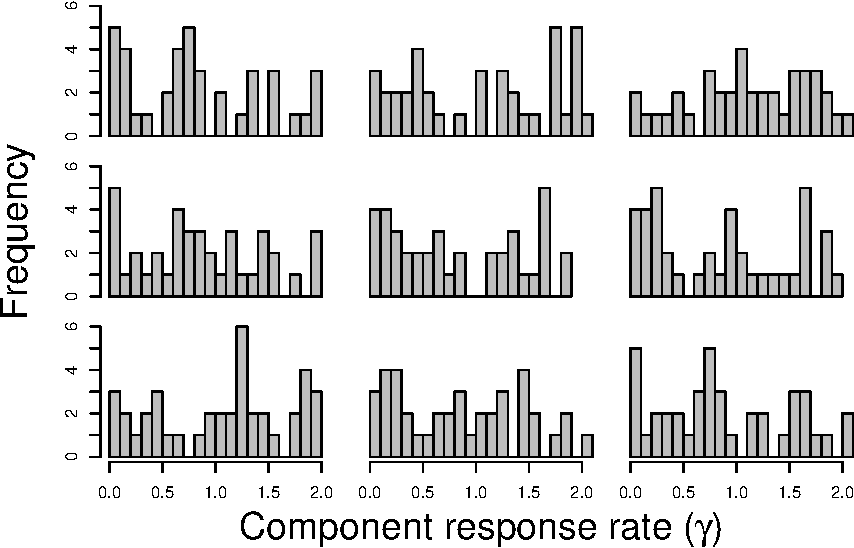
\includegraphics{unnamed-chunk-7-1.pdf}

The distribution of \(\gamma\) values found by the genetic algorithm is
uniform. A uniform distribution was used to initialise \(\gamma\)
values, so there is therefore no evidence that a particular distribution
of \(\gamma\) is likely to be found to stabilise a matrix
\(\mathbf{M}\).

\hypertarget{ecological}{\section{Stability of ecological
networks}\label{ecological}}

While the foundational work of
May\textsuperscript{\protect\hyperlink{ref-May1972}{1}} applies broadly
to complex networks, much attention has been given specifically to
ecological networks of interacting species. In these networks, the
matrix \(\mathbf{A}\) is interpreted as a community matrix and each row
and column is interpreted as a single species. The per capita effect
that the density of any species \(i\) has on the population dynamics of
species \(j\) is found in \(A_{ij}\), meaning that \(\mathbf{A}\) holds
the effects of pair-wise interactions between \(S\)
species\textsuperscript{\protect\hyperlink{ref-Allesina2012}{2},\protect\hyperlink{ref-Allesina2015}{3}}.
While May's original
work\textsuperscript{\protect\hyperlink{ref-May1972}{1}} considered only
randomly assembled communities, recent work has specifically looked at
more restricted ecological communities including competitive networks
(all off-diagonal elements of \(\mathbf{A}\) are negative), mutualist
networks (all off-diagonal elements of \(\mathbf{A}\) are positive), and
predator-prey networks (for any pair of \(i\) and \(j\), the effect of
\(i\) on \(j\) is negative and \(j\) on \(i\) is positive, or vice
versa)\textsuperscript{\protect\hyperlink{ref-Allesina2012}{2},\protect\hyperlink{ref-Allesina2015}{3}}.
In general, competitor and mutualist networks tend to be unstable, while
predator-prey networks tend to be highly
stabilising\textsuperscript{\protect\hyperlink{ref-Allesina2012}{2}}.

I investigated competitor, mutualist, and predator-prey networks
following Allesina et
al.\textsuperscript{\protect\hyperlink{ref-Allesina2012}{2}}. To create
these networks, I first generated a random matrix \(\mathbf{A}\), then
changed the elements of \(\mathbf{A}\) accordingly. If \(\mathbf{A}\)
was a competitive network, then the sign of any positive off-diagonal
elements was reversed to be negative. If \(\mathbf{A}\) was a mutualist
network, then the sign of any positive off-diagonal elements was
reversed to be positive. And if \(\mathbf{A}\) was a predator-prey
network, then all \(i\) and \(j\) pairs of elements were checked; any
pairs of the same sign were changed so that one was negative and the
other was positive.

The number of stable \(\mathbf{M = \gamma A}\) systems was estimated
\protect\hyperlink{IncrS}{exactly as it was} in the main text for random
matrices for values of \(S\) from 2 to 50 (100 in the case of the
relatively more stable predator-prey interactions), except that only
100000 random \(\mathbf{M}\) were generated instead of 1 million.

The following tables for restricted ecological communities can therefore
be compared with the random \(\mathbf{M}\)
\protect\hyperlink{IncrS}{results above} (but note that counts from
systems with comparable probabilities of stability will be an order of
magnitude lower in the tables below due to the smaller number of
\(\mathbf{M}\) matrices generated). As with the
\protect\hyperlink{IncrS}{results above}, in the tables below,
\texttt{A0} refers to matrices when \(\gamma = 1\) and \texttt{A1}
refers to matrices after \(Var(\gamma)\) is added. The column
\texttt{A0\_unstable} shows the number of \texttt{A0} matrices that are
unstable, and the column \texttt{A0\_stable} shows the number of
\texttt{A0} matrices that are stable (these two columns sum to 100000).
Similarly, the column \texttt{A1\_unstable} shows the number of
\texttt{A1} matrices that are unstable and \texttt{A1\_stable} shows the
number that are stable. The columns \texttt{A1\_stabilised} and
\texttt{A1\_destabilised} show how many \texttt{A0} matrices were
stabilised or destabilised, respectively, by \(Var(\gamma)\).

\textbf{Competition}

Results for competitor interaction networks are shown below

\begin{longtable}[]{@{}lllllll@{}}
\toprule
N & A0\_unstable & A0\_stable & A1\_unstable & A1\_stable &
A1\_stabilised & A1\_destabilised\tabularnewline
\midrule
\endhead
2 & 48 & 99952 & 48 & 99952 & 0 & 0\tabularnewline
3 & 229 & 99771 & 231 & 99769 & 0 & 2\tabularnewline
4 & 701 & 99299 & 704 & 99296 & 0 & 3\tabularnewline
5 & 1579 & 98421 & 1587 & 98413 & 0 & 8\tabularnewline
6 & 3218 & 96782 & 3253 & 96747 & 6 & 41\tabularnewline
7 & 5519 & 94481 & 5619 & 94381 & 23 & 123\tabularnewline
8 & 9062 & 90938 & 9237 & 90763 & 77 & 252\tabularnewline
9 & 13436 & 86564 & 13729 & 86271 & 230 & 523\tabularnewline
10 & 18911 & 81089 & 19303 & 80697 & 505 & 897\tabularnewline
11 & 25594 & 74406 & 25961 & 74039 & 1011 & 1378\tabularnewline
12 & 33207 & 66793 & 33382 & 66618 & 1724 & 1899\tabularnewline
13 & 41160 & 58840 & 41089 & 58911 & 2655 & 2584\tabularnewline
14 & 50575 & 49425 & 49894 & 50106 & 3777 & 3096\tabularnewline
15 & 59250 & 40750 & 57892 & 42108 & 4824 & 3466\tabularnewline
16 & 67811 & 32189 & 65740 & 34260 & 5634 & 3563\tabularnewline
17 & 75483 & 24517 & 73056 & 26944 & 5943 & 3516\tabularnewline
18 & 82551 & 17449 & 79878 & 20122 & 5780 & 3107\tabularnewline
19 & 88030 & 11970 & 85204 & 14796 & 5417 & 2591\tabularnewline
20 & 92254 & 7746 & 89766 & 10234 & 4544 & 2056\tabularnewline
21 & 95233 & 4767 & 93002 & 6998 & 3695 & 1464\tabularnewline
22 & 97317 & 2683 & 95451 & 4549 & 2803 & 937\tabularnewline
23 & 98508 & 1492 & 97122 & 2878 & 1991 & 605\tabularnewline
24 & 99240 & 760 & 98407 & 1593 & 1216 & 383\tabularnewline
25 & 99669 & 331 & 99082 & 918 & 739 & 152\tabularnewline
26 & 99871 & 129 & 99490 & 510 & 452 & 71\tabularnewline
27 & 99938 & 62 & 99732 & 268 & 240 & 34\tabularnewline
28 & 99985 & 15 & 99888 & 112 & 108 & 11\tabularnewline
29 & 99990 & 10 & 99951 & 49 & 46 & 7\tabularnewline
30 & 100000 & 0 & 99981 & 19 & 19 & 0\tabularnewline
31 & 100000 & 0 & 99993 & 7 & 7 & 0\tabularnewline
32 & 100000 & 0 & 99996 & 4 & 4 & 0\tabularnewline
33 & 100000 & 0 & 99998 & 2 & 2 & 0\tabularnewline
34 & 100000 & 0 & 100000 & 0 & 0 & 0\tabularnewline
\ldots{} & \ldots{} & \ldots{} & \ldots{} & \ldots{} & \ldots{} &
\ldots{}\tabularnewline
50 & 100000 & 0 & 100000 & 0 & 0 & 0\tabularnewline
\bottomrule
\end{longtable}

\textbf{Mutualism}

Results for mutualist interaction networks are shown below

\begin{longtable}[]{@{}lllllll@{}}
\toprule
N & A0\_unstable & A0\_stable & A1\_unstable & A1\_stable &
A1\_stabilised & A1\_destabilised\tabularnewline
\midrule
\endhead
2 & 56 & 99944 & 56 & 99944 & 0 & 0\tabularnewline
3 & 3301 & 96699 & 3301 & 96699 & 0 & 0\tabularnewline
4 & 34446 & 65554 & 34446 & 65554 & 0 & 0\tabularnewline
5 & 86520 & 13480 & 86520 & 13480 & 0 & 0\tabularnewline
6 & 99683 & 317 & 99683 & 317 & 0 & 0\tabularnewline
7 & 99998 & 2 & 99998 & 2 & 0 & 0\tabularnewline
8 & 100000 & 0 & 100000 & 0 & 0 & 0\tabularnewline
9 & 100000 & 0 & 100000 & 0 & 0 & 0\tabularnewline
10 & 100000 & 0 & 100000 & 0 & 0 & 0\tabularnewline
11 & 100000 & 0 & 100000 & 0 & 0 & 0\tabularnewline
12 & 100000 & 0 & 100000 & 0 & 0 & 0\tabularnewline
\ldots{} & \ldots{} & \ldots{} & \ldots{} & \ldots{} & \ldots{} &
\ldots{}\tabularnewline
50 & 100000 & 0 & 100000 & 0 & 0 & 0\tabularnewline
\bottomrule
\end{longtable}

\textbf{Predator-prey}

Results for predator-prey interaction networks are shown below

\begin{longtable}[]{@{}rrrrrrr@{}}
\toprule
N & A0\_unstable & A0\_stable & A1\_unstable & A1\_stable &
A1\_stabilised & A1\_destabilised\tabularnewline
\midrule
\endhead
2 & 0 & 100000 & 0 & 100000 & 0 & 0\tabularnewline
3 & 0 & 100000 & 0 & 100000 & 0 & 0\tabularnewline
4 & 0 & 100000 & 0 & 100000 & 0 & 0\tabularnewline
5 & 1 & 99999 & 1 & 99999 & 0 & 0\tabularnewline
6 & 4 & 99996 & 4 & 99996 & 0 & 0\tabularnewline
7 & 2 & 99998 & 2 & 99998 & 0 & 0\tabularnewline
8 & 5 & 99995 & 5 & 99995 & 0 & 0\tabularnewline
9 & 20 & 99980 & 21 & 99979 & 0 & 1\tabularnewline
10 & 20 & 99980 & 22 & 99978 & 0 & 2\tabularnewline
11 & 38 & 99962 & 39 & 99961 & 0 & 1\tabularnewline
12 & 64 & 99936 & 66 & 99934 & 0 & 2\tabularnewline
13 & 87 & 99913 & 91 & 99909 & 0 & 4\tabularnewline
14 & 157 & 99843 & 159 & 99841 & 0 & 2\tabularnewline
15 & 215 & 99785 & 227 & 99773 & 0 & 12\tabularnewline
16 & 293 & 99707 & 310 & 99690 & 0 & 17\tabularnewline
17 & 383 & 99617 & 408 & 99592 & 0 & 25\tabularnewline
18 & 443 & 99557 & 473 & 99527 & 3 & 33\tabularnewline
19 & 642 & 99358 & 675 & 99325 & 4 & 37\tabularnewline
20 & 836 & 99164 & 887 & 99113 & 7 & 58\tabularnewline
21 & 1006 & 98994 & 1058 & 98942 & 10 & 62\tabularnewline
22 & 1153 & 98847 & 1228 & 98772 & 20 & 95\tabularnewline
23 & 1501 & 98499 & 1593 & 98407 & 30 & 122\tabularnewline
24 & 1841 & 98159 & 1996 & 98004 & 40 & 195\tabularnewline
25 & 2146 & 97854 & 2316 & 97684 & 58 & 228\tabularnewline
26 & 2643 & 97357 & 2809 & 97191 & 119 & 285\tabularnewline
27 & 3034 & 96966 & 3258 & 96742 & 158 & 382\tabularnewline
28 & 3690 & 96310 & 3928 & 96072 & 201 & 439\tabularnewline
29 & 4257 & 95743 & 4532 & 95468 & 290 & 565\tabularnewline
30 & 4964 & 95036 & 5221 & 94779 & 424 & 681\tabularnewline
31 & 5627 & 94373 & 5978 & 94022 & 452 & 803\tabularnewline
32 & 6543 & 93457 & 6891 & 93109 & 666 & 1014\tabularnewline
33 & 7425 & 92575 & 7777 & 92223 & 818 & 1170\tabularnewline
34 & 8540 & 91460 & 8841 & 91159 & 1071 & 1372\tabularnewline
35 & 9526 & 90474 & 9842 & 90158 & 1337 & 1653\tabularnewline
36 & 10617 & 89383 & 10891 & 89109 & 1624 & 1898\tabularnewline
37 & 12344 & 87656 & 12508 & 87492 & 2021 & 2185\tabularnewline
38 & 13675 & 86325 & 13877 & 86123 & 2442 & 2644\tabularnewline
39 & 15264 & 84736 & 15349 & 84651 & 2870 & 2955\tabularnewline
40 & 17026 & 82974 & 17053 & 82947 & 3363 & 3390\tabularnewline
41 & 18768 & 81232 & 18614 & 81386 & 3905 & 3751\tabularnewline
42 & 20791 & 79209 & 20470 & 79530 & 4579 & 4258\tabularnewline
43 & 23150 & 76850 & 22754 & 77246 & 5217 & 4821\tabularnewline
44 & 25449 & 74551 & 24184 & 75816 & 6285 & 5020\tabularnewline
45 & 27702 & 72298 & 26464 & 73536 & 6754 & 5516\tabularnewline
46 & 30525 & 69475 & 28966 & 71034 & 7646 & 6087\tabularnewline
47 & 32832 & 67168 & 31125 & 68875 & 8487 & 6780\tabularnewline
48 & 36152 & 63848 & 33865 & 66135 & 9479 & 7192\tabularnewline
49 & 38714 & 61286 & 36242 & 63758 & 10125 & 7653\tabularnewline
50 & 41628 & 58372 & 38508 & 61492 & 11036 & 7916\tabularnewline
51 & 44483 & 55517 & 41023 & 58977 & 11704 & 8244\tabularnewline
52 & 48134 & 51866 & 44287 & 55713 & 12573 & 8726\tabularnewline
53 & 51138 & 48862 & 46721 & 53279 & 13223 & 8806\tabularnewline
54 & 54261 & 45739 & 49559 & 50441 & 13757 & 9055\tabularnewline
55 & 57647 & 42353 & 52403 & 47597 & 14324 & 9080\tabularnewline
56 & 60630 & 39370 & 55293 & 44707 & 14669 & 9332\tabularnewline
57 & 63647 & 36353 & 57787 & 42213 & 15103 & 9243\tabularnewline
58 & 66961 & 33039 & 60439 & 39561 & 15450 & 8928\tabularnewline
59 & 69968 & 30032 & 63708 & 36292 & 15246 & 8986\tabularnewline
60 & 72838 & 27162 & 66270 & 33730 & 15177 & 8609\tabularnewline
61 & 75609 & 24391 & 68873 & 31127 & 15006 & 8270\tabularnewline
62 & 77999 & 22001 & 71318 & 28682 & 14538 & 7857\tabularnewline
63 & 80616 & 19384 & 73517 & 26483 & 14510 & 7411\tabularnewline
64 & 83089 & 16911 & 76209 & 23791 & 13784 & 6904\tabularnewline
65 & 85150 & 14850 & 78086 & 21914 & 13412 & 6348\tabularnewline
66 & 86908 & 13092 & 80437 & 19563 & 12477 & 6006\tabularnewline
67 & 88671 & 11329 & 82379 & 17621 & 11718 & 5426\tabularnewline
68 & 90537 & 9463 & 84483 & 15517 & 10878 & 4824\tabularnewline
69 & 91969 & 8031 & 86233 & 13767 & 10033 & 4297\tabularnewline
70 & 93181 & 6819 & 87914 & 12086 & 9070 & 3803\tabularnewline
71 & 94330 & 5670 & 89200 & 10800 & 8401 & 3271\tabularnewline
72 & 95324 & 4676 & 90833 & 9167 & 7359 & 2868\tabularnewline
73 & 96143 & 3857 & 91805 & 8195 & 6726 & 2388\tabularnewline
74 & 96959 & 3041 & 93065 & 6935 & 5900 & 2006\tabularnewline
75 & 97543 & 2457 & 93987 & 6013 & 5222 & 1666\tabularnewline
76 & 97969 & 2031 & 94900 & 5100 & 4481 & 1412\tabularnewline
77 & 98497 & 1503 & 95756 & 4244 & 3809 & 1068\tabularnewline
78 & 98744 & 1256 & 96442 & 3558 & 3269 & 967\tabularnewline
79 & 99045 & 955 & 96942 & 3058 & 2837 & 734\tabularnewline
80 & 99276 & 724 & 97528 & 2472 & 2329 & 581\tabularnewline
81 & 99481 & 519 & 97996 & 2004 & 1894 & 409\tabularnewline
82 & 99556 & 444 & 98321 & 1679 & 1597 & 362\tabularnewline
83 & 99691 & 309 & 98722 & 1278 & 1227 & 258\tabularnewline
84 & 99752 & 248 & 98943 & 1057 & 1015 & 206\tabularnewline
85 & 99833 & 167 & 99144 & 856 & 837 & 148\tabularnewline
86 & 99895 & 105 & 99346 & 654 & 642 & 93\tabularnewline
87 & 99925 & 75 & 99461 & 539 & 530 & 66\tabularnewline
88 & 99945 & 55 & 99566 & 434 & 428 & 49\tabularnewline
89 & 99976 & 24 & 99675 & 325 & 324 & 23\tabularnewline
90 & 99977 & 23 & 99756 & 244 & 243 & 22\tabularnewline
91 & 99982 & 18 & 99839 & 161 & 155 & 12\tabularnewline
92 & 99988 & 12 & 99865 & 135 & 135 & 12\tabularnewline
93 & 99994 & 6 & 99885 & 115 & 115 & 6\tabularnewline
94 & 99993 & 7 & 99911 & 89 & 88 & 6\tabularnewline
95 & 99998 & 2 & 99953 & 47 & 47 & 2\tabularnewline
96 & 99999 & 1 & 99965 & 35 & 35 & 1\tabularnewline
97 & 99999 & 1 & 99979 & 21 & 21 & 1\tabularnewline
98 & 100000 & 0 & 99973 & 27 & 27 & 0\tabularnewline
99 & 100000 & 0 & 99984 & 16 & 16 & 0\tabularnewline
100 & 100000 & 0 & 99989 & 11 & 11 & 0\tabularnewline
\bottomrule
\end{longtable}

Overall, as
expected\textsuperscript{\protect\hyperlink{ref-Allesina2012}{2}},
predator-prey communities are relatively stable while mutualist
communties are highly unstable. But interestingly, while \(Var(\gamma)\)
stabilises predator-prey and competitor communities, it does not
stabilise mutualist communities. This is unsurprising because purely
mutualist communities are characterised by a very
positive\textsuperscript{\protect\hyperlink{ref-Allesina2012}{2}}
leading \(\Re(\lambda)\), and it is highly unlikely that \(Var(\gamma)\)
alone will shift all real parts of eigenvalues to negative values.

\hypertarget{connectance}{\section{Sensitivity of connectance (C)
values}\label{connectance}}

In the main text, for simplicity, I assumed connectance values of
\(C = 1\), meaning that all off-diagonal elements of a matrix
\(\mathbf{M}\) were potentially nonzero and sampled from a normal
distribution \(\mathcal{N}(0, \sigma^{2})\) where \(\sigma = 0.4\). Here
I present four tables showing the number of stable communities given
\(C = \{0.3, 0. 5, 0.7, 0.9 \}\). In all cases, uniform variation in
component response rate (\(\gamma \sim \mathcal{U}(0, 2)\)) led to a
higher number of stable communities than when \(\gamma\) did not vary
(\(\gamma = 1\)). In contrast to the main text, 100000 rather than 1
million \(\mathbf{M}\) were simulated. As with the results on
\protect\hyperlink{IncrS}{stability with increasing \(S\)} shown above,
in the tables below \texttt{A0} refers to matrices when \(\gamma = 1\),
and \texttt{A1} refers to matrices after \(Var(\gamma)\) is added. The
column \texttt{A0\_unstable} shows the number of \texttt{A0} matrices
that are unstable, and the column \texttt{A0\_stable} shows the number
of \texttt{A0} matrices that are stable (these two columns sum to
100000). Similarly, the column \texttt{A1\_unstable} shows the number of
\texttt{A1} matrices that are unstable and \texttt{A1\_stable} shows the
number that are stable. The columns \texttt{A1\_stabilised} and
\texttt{A1\_destabilised} show how many \texttt{A0} matrices were
stabilised or destabilised, respectively, by \(Var(\gamma)\).

\textbf{Connectance \(\mathbf{C = 0.3}\)}

\begin{longtable}[]{@{}llllllll@{}}
\toprule
N & A0\_unstable & A0\_stable & A1\_unstable & A1\_stable &
A1\_stabilised & A1\_destabilised & A0\_infeasible\tabularnewline
\midrule
\endhead
2 & 5 & 99995 & 5 & 99995 & 0 & 0 & 75110\tabularnewline
3 & 6 & 99994 & 6 & 99994 & 0 & 0 & 87526\tabularnewline
4 & 24 & 99976 & 24 & 99976 & 0 & 0 & 93713\tabularnewline
5 & 59 & 99941 & 59 & 99941 & 0 & 0 & 96929\tabularnewline
6 & 98 & 99902 & 98 & 99902 & 0 & 0 & 98492\tabularnewline
7 & 160 & 99840 & 161 & 99839 & 0 & 1 & 99243\tabularnewline
8 & 290 & 99710 & 293 & 99707 & 0 & 3 & 99582\tabularnewline
9 & 430 & 99570 & 434 & 99566 & 0 & 4 & 99821\tabularnewline
10 & 648 & 99352 & 653 & 99347 & 1 & 6 & 99895\tabularnewline
11 & 946 & 99054 & 957 & 99043 & 0 & 11 & 99945\tabularnewline
12 & 1392 & 98608 & 1415 & 98585 & 4 & 27 & 99978\tabularnewline
13 & 2032 & 97968 & 2065 & 97935 & 5 & 38 & 99987\tabularnewline
14 & 2627 & 97373 & 2688 & 97312 & 10 & 71 & 99988\tabularnewline
15 & 3588 & 96412 & 3647 & 96353 & 35 & 94 & 99996\tabularnewline
16 & 5019 & 94981 & 5124 & 94876 & 51 & 156 & 99998\tabularnewline
17 & 6512 & 93488 & 6673 & 93327 & 79 & 240 & 99999\tabularnewline
18 & 8444 & 91556 & 8600 & 91400 & 165 & 321 & 100000\tabularnewline
19 & 10416 & 89584 & 10667 & 89333 & 244 & 495 & 100000\tabularnewline
20 & 13254 & 86746 & 13477 & 86523 & 425 & 648 & 100000\tabularnewline
21 & 16248 & 83752 & 16481 & 83519 & 642 & 875 & 100000\tabularnewline
22 & 19497 & 80503 & 19719 & 80281 & 929 & 1151 & 100000\tabularnewline
23 & 23654 & 76346 & 23776 & 76224 & 1368 & 1490 & 100000\tabularnewline
24 & 28485 & 71515 & 28389 & 71611 & 1914 & 1818 & 100000\tabularnewline
25 & 32774 & 67226 & 32483 & 67517 & 2428 & 2137 & 100000\tabularnewline
26 & 38126 & 61874 & 37411 & 62589 & 3221 & 2506 & 100000\tabularnewline
27 & 43435 & 56565 & 42418 & 57582 & 3828 & 2811 & 100000\tabularnewline
28 & 49333 & 50667 & 47840 & 52160 & 4565 & 3072 & 100000\tabularnewline
29 & 55389 & 44611 & 53381 & 46619 & 5329 & 3321 & 100000\tabularnewline
30 & 60826 & 39174 & 58388 & 41612 & 5918 & 3480 & 100000\tabularnewline
31 & 66820 & 33180 & 64043 & 35957 & 6345 & 3568 & 100000\tabularnewline
32 & 72190 & 27810 & 69036 & 30964 & 6685 & 3531 & 100000\tabularnewline
33 & 77053 & 22947 & 73587 & 26413 & 6826 & 3360 & 100000\tabularnewline
34 & 81816 & 18184 & 78157 & 21843 & 6673 & 3014 & 100000\tabularnewline
35 & 85651 & 14349 & 82041 & 17959 & 6383 & 2773 & 100000\tabularnewline
36 & 88985 & 11015 & 85657 & 14343 & 5721 & 2393 & 100000\tabularnewline
37 & 92072 & 7928 & 88805 & 11195 & 5180 & 1913 & 100000\tabularnewline
38 & 94329 & 5671 & 91444 & 8556 & 4451 & 1566 & 100000\tabularnewline
39 & 95912 & 4088 & 93295 & 6705 & 3804 & 1187 & 100000\tabularnewline
40 & 97232 & 2768 & 95201 & 4799 & 2967 & 936 & 100000\tabularnewline
41 & 98179 & 1821 & 96506 & 3494 & 2356 & 683 & 100000\tabularnewline
42 & 98826 & 1174 & 97489 & 2511 & 1786 & 449 & 100000\tabularnewline
43 & 99275 & 725 & 98312 & 1688 & 1251 & 288 & 100000\tabularnewline
44 & 99583 & 417 & 98872 & 1128 & 903 & 192 & 100000\tabularnewline
45 & 99776 & 224 & 99339 & 661 & 576 & 139 & 100000\tabularnewline
46 & 99865 & 135 & 99518 & 482 & 413 & 66 & 100000\tabularnewline
47 & 99938 & 62 & 99744 & 256 & 226 & 32 & 100000\tabularnewline
48 & 99956 & 44 & 99824 & 176 & 151 & 19 & 100000\tabularnewline
49 & 99980 & 20 & 99914 & 86 & 85 & 19 & 100000\tabularnewline
50 & 99993 & 7 & 99950 & 50 & 46 & 3 & 100000\tabularnewline
51 & 99998 & 2 & 99971 & 29 & 28 & 1 & 100000\tabularnewline
52 & 99998 & 2 & 99986 & 14 & 14 & 2 & 100000\tabularnewline
53 & 99999 & 1 & 99992 & 8 & 7 & 0 & 100000\tabularnewline
54 & 100000 & 0 & 99997 & 3 & 3 & 0 & 100000\tabularnewline
55 & 100000 & 0 & 99999 & 1 & 1 & 0 & 100000\tabularnewline
56 & 100000 & 0 & 99998 & 2 & 2 & 0 & 100000\tabularnewline
57 & 100000 & 0 & 99999 & 1 & 1 & 0 & 100000\tabularnewline
58 & 100000 & 0 & 100000 & 0 & 0 & 0 & 100000\tabularnewline
\ldots{} & \ldots{} & \ldots{} & \ldots{} & \ldots{} & \ldots{} &
\ldots{} & \ldots{}\tabularnewline
100 & 100000 & 0 & 100000 & 0 & 0 & 0 & 100000\tabularnewline
\bottomrule
\end{longtable}

\textbf{Connectance \(\mathbf{C = 0.5}\)}

\begin{longtable}[]{@{}llllllll@{}}
\toprule
N & A0\_unstable & A0\_stable & A1\_unstable & A1\_stable &
A1\_stabilised & A1\_destabilised & A0\_infeasible\tabularnewline
\midrule
\endhead
2 & 7 & 99993 & 7 & 99993 & 0 & 0 & 74863\tabularnewline
3 & 32 & 99968 & 32 & 99968 & 0 & 0 & 87434\tabularnewline
4 & 122 & 99878 & 122 & 99878 & 0 & 0 & 93761\tabularnewline
5 & 320 & 99680 & 321 & 99679 & 0 & 1 & 96830\tabularnewline
6 & 667 & 99333 & 673 & 99327 & 0 & 6 & 98481\tabularnewline
7 & 1233 & 98767 & 1252 & 98748 & 0 & 19 & 99187\tabularnewline
8 & 2123 & 97877 & 2156 & 97844 & 3 & 36 & 99654\tabularnewline
9 & 3415 & 96585 & 3471 & 96529 & 16 & 72 & 99816\tabularnewline
10 & 5349 & 94651 & 5450 & 94550 & 30 & 131 & 99900\tabularnewline
11 & 7990 & 92010 & 8185 & 91815 & 81 & 276 & 99958\tabularnewline
12 & 11073 & 88927 & 11301 & 88699 & 219 & 447 & 99973\tabularnewline
13 & 14971 & 85029 & 15204 & 84796 & 445 & 678 & 99986\tabularnewline
14 & 19754 & 80246 & 19992 & 80008 & 764 & 1002 & 99991\tabularnewline
15 & 25020 & 74980 & 25239 & 74761 & 1185 & 1404 & 99996\tabularnewline
16 & 30860 & 69140 & 30938 & 69062 & 1902 & 1980 & 99999\tabularnewline
17 & 37844 & 62156 & 37562 & 62438 & 2758 & 2476 & 100000\tabularnewline
18 & 44909 & 55091 & 44251 & 55749 & 3595 & 2937 & 99999\tabularnewline
19 & 52322 & 47678 & 51011 & 48989 & 4573 & 3262 & 99999\tabularnewline
20 & 60150 & 39850 & 58295 & 41705 & 5382 & 3527 & 100000\tabularnewline
21 & 67147 & 32853 & 64895 & 35105 & 5925 & 3673 & 100000\tabularnewline
22 & 74177 & 25823 & 71358 & 28642 & 6310 & 3491 & 100000\tabularnewline
23 & 80297 & 19703 & 77034 & 22966 & 6507 & 3244 & 100000\tabularnewline
24 & 85372 & 14628 & 82039 & 17961 & 6209 & 2876 & 100000\tabularnewline
25 & 89719 & 10281 & 86539 & 13461 & 5562 & 2382 & 100000\tabularnewline
26 & 92947 & 7053 & 90141 & 9859 & 4707 & 1901 & 100000\tabularnewline
27 & 95436 & 4564 & 92950 & 7050 & 3844 & 1358 & 100000\tabularnewline
28 & 97196 & 2804 & 95171 & 4829 & 2999 & 974 & 100000\tabularnewline
29 & 98300 & 1700 & 96842 & 3158 & 2115 & 657 & 100000\tabularnewline
30 & 99103 & 897 & 98033 & 1967 & 1466 & 396 & 100000\tabularnewline
31 & 99502 & 498 & 98665 & 1335 & 1068 & 231 & 100000\tabularnewline
32 & 99745 & 255 & 99185 & 815 & 696 & 136 & 100000\tabularnewline
33 & 99881 & 119 & 99572 & 428 & 375 & 66 & 100000\tabularnewline
34 & 99955 & 45 & 99788 & 212 & 191 & 24 & 100000\tabularnewline
35 & 99979 & 21 & 99900 & 100 & 95 & 16 & 100000\tabularnewline
36 & 99995 & 5 & 99950 & 50 & 50 & 5 & 100000\tabularnewline
37 & 99997 & 3 & 99970 & 30 & 28 & 1 & 100000\tabularnewline
38 & 99998 & 2 & 99986 & 14 & 13 & 1 & 100000\tabularnewline
39 & 99999 & 1 & 99991 & 9 & 9 & 1 & 100000\tabularnewline
40 & 100000 & 0 & 100000 & 0 & 0 & 0 & 100000\tabularnewline
41 & 100000 & 0 & 99999 & 1 & 1 & 0 & 100000\tabularnewline
42 & 100000 & 0 & 99999 & 1 & 1 & 0 & 100000\tabularnewline
43 & 100000 & 0 & 100000 & 0 & 0 & 0 & 100000\tabularnewline
\ldots{} & \ldots{} & \ldots{} & \ldots{} & \ldots{} & \ldots{} &
\ldots{} & \ldots{}\tabularnewline
50 & 100000 & 0 & 100000 & 0 & 0 & 0 & 100000\tabularnewline
\bottomrule
\end{longtable}

\textbf{Connectance \(\mathbf{C = 0.7}\)}

\begin{longtable}[]{@{}llllllll@{}}
\toprule
N & A0\_unstable & A0\_stable & A1\_unstable & A1\_stable &
A1\_stabilised & A1\_destabilised & A0\_infeasible\tabularnewline
\midrule
\endhead
2 & 7 & 99993 & 7 & 99993 & 0 & 0 & 75160\tabularnewline
3 & 106 & 99894 & 106 & 99894 & 0 & 0 & 87447\tabularnewline
4 & 395 & 99605 & 397 & 99603 & 0 & 2 & 93849\tabularnewline
5 & 1117 & 98883 & 1123 & 98877 & 0 & 6 & 96827\tabularnewline
6 & 2346 & 97654 & 2367 & 97633 & 6 & 27 & 98402\tabularnewline
7 & 4314 & 95686 & 4388 & 95612 & 16 & 90 & 99218\tabularnewline
8 & 7327 & 92673 & 7456 & 92544 & 61 & 190 & 99611\tabularnewline
9 & 11514 & 88486 & 11792 & 88208 & 150 & 428 & 99808\tabularnewline
10 & 16247 & 83753 & 16584 & 83416 & 415 & 752 & 99904\tabularnewline
11 & 22481 & 77519 & 22759 & 77241 & 884 & 1162 & 99952\tabularnewline
12 & 29459 & 70541 & 29729 & 70271 & 1548 & 1818 & 99977\tabularnewline
13 & 37631 & 62369 & 37567 & 62433 & 2419 & 2355 & 99984\tabularnewline
14 & 46317 & 53683 & 45696 & 54304 & 3548 & 2927 & 99995\tabularnewline
15 & 54945 & 45055 & 53695 & 46305 & 4671 & 3421 & 99994\tabularnewline
16 & 63683 & 36317 & 61643 & 38357 & 5567 & 3527 & 99999\tabularnewline
17 & 72004 & 27996 & 69375 & 30625 & 6124 & 3495 & 100000\tabularnewline
18 & 79220 & 20780 & 76158 & 23842 & 6413 & 3351 & 100000\tabularnewline
19 & 85286 & 14714 & 82283 & 17717 & 5982 & 2979 & 99999\tabularnewline
20 & 90240 & 9760 & 87181 & 12819 & 5398 & 2339 & 100000\tabularnewline
21 & 93676 & 6324 & 91077 & 8923 & 4468 & 1869 & 100000\tabularnewline
22 & 96203 & 3797 & 94045 & 5955 & 3425 & 1267 & 100000\tabularnewline
23 & 97866 & 2134 & 96161 & 3839 & 2496 & 791 & 100000\tabularnewline
24 & 98842 & 1158 & 97633 & 2367 & 1713 & 504 & 100000\tabularnewline
25 & 99433 & 567 & 98630 & 1370 & 1079 & 276 & 100000\tabularnewline
26 & 99760 & 240 & 99259 & 741 & 655 & 154 & 100000\tabularnewline
27 & 99895 & 105 & 99576 & 424 & 377 & 58 & 100000\tabularnewline
28 & 99950 & 50 & 99790 & 210 & 194 & 34 & 100000\tabularnewline
29 & 99981 & 19 & 99915 & 85 & 80 & 14 & 100000\tabularnewline
30 & 99994 & 6 & 99952 & 48 & 47 & 5 & 100000\tabularnewline
31 & 99998 & 2 & 99972 & 28 & 28 & 2 & 100000\tabularnewline
32 & 99999 & 1 & 99992 & 8 & 8 & 1 & 100000\tabularnewline
33 & 100000 & 0 & 99997 & 3 & 3 & 0 & 100000\tabularnewline
34 & 100000 & 0 & 99999 & 1 & 1 & 0 & 100000\tabularnewline
35 & 100000 & 0 & 100000 & 0 & 0 & 0 & 100000\tabularnewline
\ldots{} & \ldots{} & \ldots{} & \ldots{} & \ldots{} & \ldots{} &
\ldots{} & \ldots{}\tabularnewline
50 & 100000 & 0 & 100000 & 0 & 0 & 0 & 100000\tabularnewline
\bottomrule
\end{longtable}

\textbf{Connectance \(\mathbf{C = 0.9}\)}

\begin{longtable}[]{@{}llllllll@{}}
\toprule
N & A0\_unstable & A0\_stable & A1\_unstable & A1\_stable &
A1\_stabilised & A1\_destabilised & A0\_infeasible\tabularnewline
\midrule
\endhead
2 & 14 & 99986 & 14 & 99986 & 0 & 0 & 75187\tabularnewline
3 & 240 & 99760 & 240 & 99760 & 0 & 0 & 87443\tabularnewline
4 & 1008 & 98992 & 1016 & 98984 & 0 & 8 & 93795\tabularnewline
5 & 2708 & 97292 & 2729 & 97271 & 2 & 23 & 96814\tabularnewline
6 & 5669 & 94331 & 5755 & 94245 & 13 & 99 & 98439\tabularnewline
7 & 9848 & 90152 & 10057 & 89943 & 91 & 300 & 99208\tabularnewline
8 & 15903 & 84097 & 16201 & 83799 & 336 & 634 & 99603\tabularnewline
9 & 22707 & 77293 & 23110 & 76890 & 765 & 1168 & 99803\tabularnewline
10 & 30796 & 69204 & 31122 & 68878 & 1526 & 1852 & 99909\tabularnewline
11 & 40224 & 59776 & 40082 & 59918 & 2649 & 2507 & 99951\tabularnewline
12 & 49934 & 50066 & 49288 & 50712 & 3773 & 3127 & 99977\tabularnewline
13 & 60138 & 39862 & 58803 & 41197 & 4984 & 3649 & 99986\tabularnewline
14 & 69100 & 30900 & 67110 & 32890 & 5755 & 3765 & 99995\tabularnewline
15 & 77607 & 22393 & 74884 & 25116 & 6273 & 3550 & 100000\tabularnewline
16 & 84663 & 15337 & 81780 & 18220 & 5975 & 3092 & 100000\tabularnewline
17 & 90075 & 9925 & 87290 & 12710 & 5209 & 2424 & 100000\tabularnewline
18 & 93944 & 6056 & 91419 & 8581 & 4271 & 1746 & 100000\tabularnewline
19 & 96650 & 3350 & 94530 & 5470 & 3287 & 1167 & 99999\tabularnewline
20 & 98160 & 1840 & 96698 & 3302 & 2191 & 729 & 100000\tabularnewline
21 & 99111 & 889 & 98133 & 1867 & 1389 & 411 & 100000\tabularnewline
22 & 99588 & 412 & 98905 & 1095 & 903 & 220 & 100000\tabularnewline
23 & 99837 & 163 & 99480 & 520 & 452 & 95 & 100000\tabularnewline
24 & 99932 & 68 & 99744 & 256 & 228 & 40 & 100000\tabularnewline
25 & 99976 & 24 & 99863 & 137 & 133 & 20 & 100000\tabularnewline
26 & 99995 & 5 & 99950 & 50 & 49 & 4 & 100000\tabularnewline
27 & 99996 & 4 & 99986 & 14 & 13 & 3 & 100000\tabularnewline
28 & 100000 & 0 & 99993 & 7 & 7 & 0 & 100000\tabularnewline
29 & 100000 & 0 & 99996 & 4 & 4 & 0 & 100000\tabularnewline
30 & 100000 & 0 & 99998 & 2 & 2 & 0 & 100000\tabularnewline
31 & 100000 & 0 & 100000 & 0 & 0 & 0 & 100000\tabularnewline
\ldots{} & \ldots{} & \ldots{} & \ldots{} & \ldots{} & \ldots{} &
\ldots{} & \ldots{}\tabularnewline
50 & 100000 & 0 & 100000 & 0 & 0 & 0 & 100000\tabularnewline
\bottomrule
\end{longtable}

\hypertarget{sigma}{\section{\texorpdfstring{Sensitivity of interaction
strength (\(\sigma\))
values}{Sensitivity of interaction strength (\textbackslash{}sigma) values}}\label{sigma}}

Results below show stability results given varying interaction strengths
(\(\sigma\)) for \(C = 0.05\) (note that system size \(S\) values are
larger and increase by 10 with increasing rows). In the tables below (as
\protect\hyperlink{IncrS}{above}), \texttt{A0} and \texttt{A1} refers to
matrices for \(\gamma = 1\) and \(Var(\gamma)\), respectively.

\textbf{Interaction strength \(\mathbf{\sigma = 0.3}\)}

\begin{longtable}[]{@{}rrrrrrr@{}}
\toprule
S & A0\_unstable & A0\_stable & A1\_unstable & A1\_stable &
A1\_stabilised & A1\_destabilised\tabularnewline
\midrule
\endhead
10 & 0 & 100000 & 0 & 100000 & 0 & 0\tabularnewline
20 & 0 & 100000 & 0 & 100000 & 0 & 0\tabularnewline
30 & 0 & 100000 & 0 & 100000 & 0 & 0\tabularnewline
40 & 0 & 100000 & 0 & 100000 & 0 & 0\tabularnewline
50 & 0 & 100000 & 0 & 100000 & 0 & 0\tabularnewline
60 & 2 & 99998 & 2 & 99998 & 0 & 0\tabularnewline
70 & 4 & 99996 & 4 & 99996 & 0 & 0\tabularnewline
80 & 6 & 99994 & 6 & 99994 & 0 & 0\tabularnewline
90 & 5 & 99995 & 5 & 99995 & 0 & 0\tabularnewline
100 & 11 & 99989 & 11 & 99989 & 0 & 0\tabularnewline
110 & 12 & 99988 & 13 & 99987 & 0 & 1\tabularnewline
120 & 23 & 99977 & 23 & 99977 & 0 & 0\tabularnewline
130 & 40 & 99960 & 40 & 99960 & 0 & 0\tabularnewline
140 & 62 & 99938 & 65 & 99935 & 0 & 3\tabularnewline
150 & 162 & 99838 & 165 & 99835 & 0 & 3\tabularnewline
160 & 325 & 99675 & 329 & 99671 & 2 & 6\tabularnewline
170 & 829 & 99171 & 851 & 99149 & 6 & 28\tabularnewline
180 & 1817 & 98183 & 1860 & 98140 & 31 & 74\tabularnewline
190 & 3927 & 96073 & 3989 & 96011 & 143 & 205\tabularnewline
200 & 8084 & 91916 & 8048 & 91952 & 557 & 521\tabularnewline
210 & 15558 & 84442 & 15147 & 84853 & 1534 & 1123\tabularnewline
220 & 26848 & 73152 & 25342 & 74658 & 3625 & 2119\tabularnewline
230 & 43386 & 56614 & 39535 & 60465 & 6992 & 3141\tabularnewline
240 & 62734 & 37266 & 56684 & 43316 & 9815 & 3765\tabularnewline
250 & 80128 & 19872 & 73080 & 26920 & 10128 & 3080\tabularnewline
260 & 92206 & 7794 & 86619 & 13381 & 7490 & 1903\tabularnewline
270 & 97946 & 2054 & 94824 & 5176 & 3797 & 675\tabularnewline
280 & 99659 & 341 & 98534 & 1466 & 1265 & 140\tabularnewline
290 & 99962 & 38 & 99696 & 304 & 281 & 15\tabularnewline
300 & 99994 & 6 & 99964 & 36 & 34 & 4\tabularnewline
\bottomrule
\end{longtable}

\textbf{Interaction strength \(\mathbf{\sigma = 0.4}\)}

\begin{longtable}[]{@{}lllllll@{}}
\toprule
S & A0\_unstable & A0\_stable & A1\_unstable & A1\_stable &
A1\_stabilised & A1\_destabilised\tabularnewline
\midrule
\endhead
10 & 3 & 99997 & 3 & 99997 & 0 & 0\tabularnewline
20 & 15 & 99985 & 15 & 99985 & 0 & 0\tabularnewline
30 & 48 & 99952 & 48 & 99952 & 0 & 0\tabularnewline
40 & 85 & 99915 & 85 & 99915 & 0 & 0\tabularnewline
50 & 163 & 99837 & 163 & 99837 & 0 & 0\tabularnewline
60 & 280 & 99720 & 282 & 99718 & 0 & 2\tabularnewline
70 & 561 & 99439 & 566 & 99434 & 3 & 8\tabularnewline
80 & 1009 & 98991 & 1029 & 98971 & 6 & 26\tabularnewline
90 & 2126 & 97874 & 2175 & 97825 & 31 & 80\tabularnewline
100 & 4580 & 95420 & 4653 & 95347 & 142 & 215\tabularnewline
110 & 9540 & 90460 & 9632 & 90368 & 465 & 557\tabularnewline
120 & 19090 & 80910 & 18668 & 81332 & 1676 & 1254\tabularnewline
130 & 35047 & 64953 & 33220 & 66780 & 4172 & 2345\tabularnewline
140 & 56411 & 43589 & 52439 & 47561 & 7297 & 3325\tabularnewline
150 & 78003 & 21997 & 72574 & 27426 & 8477 & 3048\tabularnewline
160 & 92678 & 7322 & 88438 & 11562 & 5901 & 1661\tabularnewline
170 & 98614 & 1386 & 96670 & 3330 & 2397 & 453\tabularnewline
180 & 99839 & 161 & 99418 & 582 & 499 & 78\tabularnewline
190 & 99990 & 10 & 99945 & 55 & 52 & 7\tabularnewline
200 & 100000 & 0 & 99995 & 5 & 5 & 0\tabularnewline
210 & 100000 & 0 & 100000 & 0 & 0 & 0\tabularnewline
\ldots{} & \ldots{} & \ldots{} & \ldots{} & \ldots{} & \ldots{} &
\ldots{}\tabularnewline
300 & 100000 & 0 & 100000 & 0 & 0 & 0\tabularnewline
\bottomrule
\end{longtable}

\textbf{Interaction strength \(\mathbf{\sigma = 0.5}\)}

\begin{longtable}[]{@{}lllllll@{}}
\toprule
S & A0\_unstable & A0\_stable & A1\_unstable & A1\_stable &
A1\_stabilised & A1\_destabilised\tabularnewline
\midrule
\endhead
10 & 36 & 99964 & 36 & 99964 & 0 & 0\tabularnewline
20 & 195 & 99805 & 195 & 99805 & 0 & 0\tabularnewline
30 & 519 & 99481 & 523 & 99477 & 0 & 4\tabularnewline
40 & 1096 & 98904 & 1101 & 98899 & 2 & 7\tabularnewline
50 & 2375 & 97625 & 2397 & 97603 & 9 & 31\tabularnewline
60 & 4898 & 95102 & 4968 & 95032 & 83 & 153\tabularnewline
70 & 10841 & 89159 & 10916 & 89084 & 432 & 507\tabularnewline
80 & 22281 & 77719 & 21988 & 78012 & 1622 & 1329\tabularnewline
90 & 42010 & 57990 & 39998 & 60002 & 4458 & 2446\tabularnewline
100 & 67289 & 32711 & 63098 & 36902 & 7153 & 2962\tabularnewline
110 & 88137 & 11863 & 84023 & 15977 & 6108 & 1994\tabularnewline
120 & 97678 & 2322 & 95557 & 4443 & 2740 & 619\tabularnewline
130 & 99795 & 205 & 99304 & 696 & 578 & 87\tabularnewline
140 & 99989 & 11 & 99948 & 52 & 49 & 8\tabularnewline
150 & 100000 & 0 & 100000 & 0 & 0 & 0\tabularnewline
\ldots{} & \ldots{} & \ldots{} & \ldots{} & \ldots{} & \ldots{} &
\ldots{}\tabularnewline
300 & 100000 & 0 & 100000 & 0 & 0 & 0\tabularnewline
\bottomrule
\end{longtable}

\textbf{Interaction strength \(\mathbf{\sigma = 0.6}\)}

\begin{longtable}[]{@{}lllllll@{}}
\toprule
S & A0\_unstable & A0\_stable & A1\_unstable & A1\_stable &
A1\_stabilised & A1\_destabilised\tabularnewline
\midrule
\endhead
10 & 162 & 99838 & 162 & 99838 & 0 & 0\tabularnewline
20 & 798 & 99202 & 799 & 99201 & 0 & 1\tabularnewline
30 & 2273 & 97727 & 2289 & 97711 & 6 & 22\tabularnewline
40 & 5259 & 94741 & 5298 & 94702 & 70 & 109\tabularnewline
50 & 12084 & 87916 & 12054 & 87946 & 446 & 416\tabularnewline
60 & 26072 & 73928 & 25511 & 74489 & 1810 & 1249\tabularnewline
70 & 50121 & 49879 & 47747 & 52253 & 4748 & 2374\tabularnewline
80 & 77806 & 22194 & 73810 & 26190 & 6421 & 2425\tabularnewline
90 & 94862 & 5138 & 92069 & 7931 & 3842 & 1049\tabularnewline
100 & 99527 & 473 & 98822 & 1178 & 870 & 165\tabularnewline
110 & 99984 & 16 & 99912 & 88 & 80 & 8\tabularnewline
120 & 100000 & 0 & 99998 & 2 & 2 & 0\tabularnewline
130 & 100000 & 0 & 100000 & 0 & 0 & 0\tabularnewline
\ldots{} & \ldots{} & \ldots{} & \ldots{} & \ldots{} & \ldots{} &
\ldots{}\tabularnewline
300 & 100000 & 0 & 100000 & 0 & 0 & 0\tabularnewline
\bottomrule
\end{longtable}

\hypertarget{gam_dist}{\section{\texorpdfstring{Sensitivity of
distribution of
\(\gamma\)}{Sensitivity of distribution of \textbackslash{}gamma}}\label{gam_dist}}

In the main text, I considered a uniform distribution of component
response rates \(\gamma \sim \mathcal{U}(0, 2)\). The number of unstable
and stable \(\mathbf{M}\) matrices are reported in
\protect\hyperlink{IncrS}{a table above} across different values of
\(S\). Here I show complementary results for three different
distributions including an exponential, beta, and gamma distribution of
\(\gamma\) values. The shape of these distributions is shown in the
figure below.

\begin{center}\rule{0.5\linewidth}{\linethickness}\end{center}

\textbf{Distributions of component response rate
(\(\boldsymbol{\gamma}\)) values in complex systems.} The stabilities of
simulated complex systems with these \(\gamma\) distributions are
compared to otherwise identical complex systems with a fixed component
response rate of \(\gamma = 1\) across different system sizes (\(S\);
i.e., component numbers) given a unit \(\gamma\) standard deviation
(\(\sigma_{\gamma} = 1\)) for b-d. Distributions are as follows: (a)
uniform, (b) exponential, (c) beta (\(\alpha = 0.5\) and
\(\beta = 0.5\)), and (d) gamma (\(k = 2\) and \(\theta = 2\)). Each
panel shows 1 million randomly generated \(\gamma\) values.

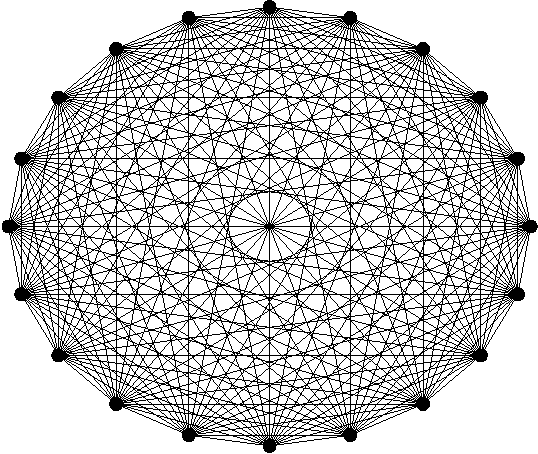
\includegraphics{unnamed-chunk-23-1.pdf}

\begin{center}\rule{0.5\linewidth}{\linethickness}\end{center}

The same 100000 \(\mathbf{M}\) matrices were used to investigate
stability when applying each of these different distributions of
\(\gamma\) values. The table below shows the number of \(\mathbf{M}\)
that were unstable (\_unst) and stable (\_stbl) for the exponential
(Exp), beta, and gamma distributions.

\begin{Shaded}
\begin{Highlighting}[]
\NormalTok{fourdists <-}\StringTok{ }\KeywordTok{read.csv}\NormalTok{(}\DataTypeTok{file =} \StringTok{"sim_results/different_distr/four_distr_rand.csv"}\NormalTok{);}
\KeywordTok{kable}\NormalTok{(fourdists);}
\end{Highlighting}
\end{Shaded}

\begin{longtable}[]{@{}lllllll@{}}
\toprule
S & Exp\_unst & Exp\_stbl & beta\_unst & beta\_stbl & gamma\_unst &
gamma\_stbl\tabularnewline
\midrule
\endhead
2 & 30 & 99970 & 30 & 99970 & 30 & 99970\tabularnewline
3 & 355 & 99645 & 355 & 99645 & 355 & 99645\tabularnewline
4 & 1506 & 98494 & 1512 & 98488 & 1516 & 98484\tabularnewline
5 & 3930 & 96070 & 3971 & 96029 & 4006 & 95994\tabularnewline
6 & 7738 & 92262 & 7844 & 92156 & 7918 & 92082\tabularnewline
7 & 13606 & 86394 & 13889 & 86111 & 13990 & 86010\tabularnewline
8 & 20535 & 79465 & 21002 & 78998 & 21114 & 78886\tabularnewline
9 & 28614 & 71386 & 29060 & 70940 & 29110 & 70890\tabularnewline
10 & 38375 & 61625 & 38388 & 61612 & 38441 & 61559\tabularnewline
11 & 48616 & 51384 & 48211 & 51789 & 47957 & 52043\tabularnewline
12 & 59254 & 40746 & 58025 & 41975 & 57473 & 42527\tabularnewline
13 & 68816 & 31184 & 66753 & 33247 & 66127 & 33873\tabularnewline
14 & 77721 & 22279 & 75149 & 24851 & 74222 & 25778\tabularnewline
15 & 84842 & 15158 & 82030 & 17970 & 81040 & 18960\tabularnewline
16 & 90365 & 9635 & 87809 & 12191 & 86600 & 13400\tabularnewline
17 & 94171 & 5829 & 91756 & 8244 & 90668 & 9332\tabularnewline
18 & 96978 & 3022 & 94977 & 5023 & 94176 & 5824\tabularnewline
19 & 98376 & 1624 & 97018 & 2982 & 96268 & 3732\tabularnewline
20 & 99218 & 782 & 98357 & 1643 & 97765 & 2235\tabularnewline
21 & 99678 & 322 & 99124 & 876 & 98746 & 1254\tabularnewline
22 & 99864 & 136 & 99599 & 401 & 99323 & 677\tabularnewline
23 & 99954 & 46 & 99783 & 217 & 99668 & 332\tabularnewline
24 & 99978 & 22 & 99920 & 80 & 99821 & 179\tabularnewline
25 & 99996 & 4 & 99967 & 33 & 99911 & 89\tabularnewline
26 & 99999 & 1 & 99979 & 21 & 99960 & 40\tabularnewline
27 & 99999 & 1 & 99990 & 10 & 99983 & 17\tabularnewline
28 & 100000 & 0 & 99999 & 1 & 99991 & 9\tabularnewline
29 & 100000 & 0 & 99999 & 1 & 99999 & 1\tabularnewline
30 & 100000 & 0 & 100000 & 0 & 100000 & 0\tabularnewline
31 & 100000 & 0 & 100000 & 0 & 99999 & 1\tabularnewline
32 & 100000 & 0 & 100000 & 0 & 100000 & 0\tabularnewline
\ldots{} & \ldots{} & \ldots{} & \ldots{} & \ldots{} & \ldots{} &
\ldots{}\tabularnewline
50 & 100000 & 0 & 100000 & 0 & 100000 & 0\tabularnewline
\bottomrule
\end{longtable}

In comparison to the uniform distribution (a), proportionally fewer
random systems are found with the exponential distribution (b), while
more are found with the beta (c) and gamma (d) distributions.

\hypertarget{Feasibility}{\section{Feasibility of complex
systems}\label{Feasibility}}

When feasibility was evaluated with and without variation in \(\gamma\),
there was no increase in stability for \(\mathbf{M}\) where \(\gamma\)
varied as compared to where \(\gamma = 1\). Results below illustrate
this result, which was general to all other simulations performed.

\begin{longtable}[]{@{}rrrrrrr@{}}
\toprule
S & A0\_infeasible & A0\_feasible & A1\_infeasible & A1\_feasible &
A1\_made\_feasible & A1\_made\_infeasible\tabularnewline
\midrule
\endhead
2 & 749978 & 250022 & 749942 & 250058 & 35552 & 35516\tabularnewline
3 & 874519 & 125481 & 874296 & 125704 & 36803 & 36580\tabularnewline
4 & 937192 & 62808 & 937215 & 62785 & 26440 & 26463\tabularnewline
5 & 968776 & 31224 & 968639 & 31361 & 16319 & 16182\tabularnewline
6 & 984313 & 15687 & 984463 & 15537 & 9006 & 9156\tabularnewline
7 & 992149 & 7851 & 992161 & 7839 & 4991 & 5003\tabularnewline
8 & 996124 & 3876 & 996103 & 3897 & 2644 & 2623\tabularnewline
9 & 998014 & 1986 & 998027 & 1973 & 1361 & 1374\tabularnewline
10 & 999031 & 969 & 999040 & 960 & 698 & 707\tabularnewline
11 & 999546 & 454 & 999514 & 486 & 377 & 345\tabularnewline
12 & 999764 & 236 & 999792 & 208 & 160 & 188\tabularnewline
13 & 999883 & 117 & 999865 & 135 & 105 & 87\tabularnewline
14 & 999938 & 62 & 999945 & 55 & 40 & 47\tabularnewline
15 & 999971 & 29 & 999964 & 36 & 31 & 24\tabularnewline
16 & 999988 & 12 & 999991 & 9 & 8 & 11\tabularnewline
17 & 999996 & 4 & 999991 & 9 & 8 & 3\tabularnewline
18 & 999997 & 3 & 999999 & 1 & 1 & 3\tabularnewline
19 & 999998 & 2 & 999997 & 3 & 3 & 2\tabularnewline
20 & 1000000 & 0 & 999999 & 1 & 1 & 0\tabularnewline
21 & 1000000 & 0 & 1000000 & 0 & 0 & 0\tabularnewline
22 & 999999 & 1 & 1000000 & 0 & 0 & 1\tabularnewline
23 & 1000000 & 0 & 1000000 & 0 & 0 & 0\tabularnewline
24 & 1000000 & 0 & 1000000 & 0 & 0 & 0\tabularnewline
25 & 1000000 & 0 & 1000000 & 0 & 0 & 0\tabularnewline
26 & 1000000 & 0 & 1000000 & 0 & 0 & 0\tabularnewline
27 & 1000000 & 0 & 1000000 & 0 & 0 & 0\tabularnewline
28 & 1000000 & 0 & 1000000 & 0 & 0 & 0\tabularnewline
29 & 1000000 & 0 & 1000000 & 0 & 0 & 0\tabularnewline
30 & 1000000 & 0 & 1000000 & 0 & 0 & 0\tabularnewline
31 & 1000000 & 0 & 1000000 & 0 & 0 & 0\tabularnewline
32 & 1000000 & 0 & 1000000 & 0 & 0 & 0\tabularnewline
33 & 1000000 & 0 & 1000000 & 0 & 0 & 0\tabularnewline
34 & 1000000 & 0 & 1000000 & 0 & 0 & 0\tabularnewline
35 & 1000000 & 0 & 1000000 & 0 & 0 & 0\tabularnewline
36 & 1000000 & 0 & 1000000 & 0 & 0 & 0\tabularnewline
37 & 1000000 & 0 & 1000000 & 0 & 0 & 0\tabularnewline
38 & 1000000 & 0 & 1000000 & 0 & 0 & 0\tabularnewline
39 & 1000000 & 0 & 1000000 & 0 & 0 & 0\tabularnewline
40 & 1000000 & 0 & 1000000 & 0 & 0 & 0\tabularnewline
41 & 1000000 & 0 & 1000000 & 0 & 0 & 0\tabularnewline
42 & 1000000 & 0 & 1000000 & 0 & 0 & 0\tabularnewline
43 & 1000000 & 0 & 1000000 & 0 & 0 & 0\tabularnewline
44 & 1000000 & 0 & 1000000 & 0 & 0 & 0\tabularnewline
45 & 1000000 & 0 & 1000000 & 0 & 0 & 0\tabularnewline
46 & 1000000 & 0 & 1000000 & 0 & 0 & 0\tabularnewline
47 & 1000000 & 0 & 1000000 & 0 & 0 & 0\tabularnewline
48 & 1000000 & 0 & 1000000 & 0 & 0 & 0\tabularnewline
49 & 1000000 & 0 & 1000000 & 0 & 0 & 0\tabularnewline
50 & 1000000 & 0 & 1000000 & 0 & 0 & 0\tabularnewline
\bottomrule
\end{longtable}

Hence, in general, \(Var(\gamma)\) does not appear to affect feasibility
in pure species interaction networks.

\section*{References}\label{references}
\addcontentsline{toc}{section}{References}

\hypertarget{refs}{}
\hypertarget{ref-May1972}{}
1. May, R. M. Will a large complex system be stable? \emph{Nature}
\textbf{238,} 413--414 (1972).

\hypertarget{ref-Allesina2012}{}
2. Allesina, S. \& Tang, S. Stability criteria for complex ecosystems.
\emph{Nature} \textbf{483,} 205--208 (2012).

\hypertarget{ref-Allesina2015}{}
3. Allesina, S. \emph{et al.} Predicting the stability of large
structured food webs. \emph{Nature Communications} \textbf{6,} 7842
(2015).


\end{document}
